\documentclass[conference,a4paper]{IEEEtran}
\pdfminorversion=6
\usepackage[T1]{fontenc}
\usepackage[utf8]{inputenc}
\usepackage{graphicx,booktabs,tabularx,amsmath,amssymb,tikz,cite}
\usepackage[table]{xcolor}
\usepackage{pgfplots}
\pgfplotsset{compat=1.18}
\usepgfplotslibrary{groupplots}
\usepackage[hidelinks]{hyperref}
\newcolumntype{Y}{>{\raggedright\arraybackslash}X}
\newcommand{\ind}{\mathbf{1}}
\begin{document}
\title{XBone-Net: Parameter-Efficient Radiograph Classification with Clinical History}
\author{\IEEEauthorblockN{%
Van-Le-Ba-Thanh Nguyen\textsuperscript{1,2},
Gia-Kiet Nguyen\textsuperscript{1,2},
Quoc-Ngoc Ly\textsuperscript{1,2},
Thi-Thanh-Ha Do\textsuperscript{1,2}}
\IEEEauthorblockA{%
\textsuperscript{1}Faculty of Information Technology, University of Science, Vietnam\\
\textsuperscript{2}Vietnam National University, Ho Chi Minh City, Vietnam\\
\{nvlbthanh22, ngkiet22\}@clc.fitus.edu.vn\\
\{lqngoc, dttha\}@fit.hcmus.edu.vn}}
\maketitle

\begin{abstract}
Clinical history complements skeletal radiographs, but adapting biomedical vision--language models to small, imbalanced cohorts requires effective fusion under limited training resources. Existing image--text pretraining provides transferable representations, while the downstream trade-off between classification performance and adaptation cost remains task dependent. We present XBone-Net, a parameter-efficient framework built on BiomedCLIP. A first stage learns low-rank adapters through class-aware soft image--text alignment, followed by a second stage that combines native tokens using bidirectional global-to-local cross-attention and class-balanced classification. Across three training seeds, XBone-Net achieves Macro-F1 of $0.5727\pm0.0193$ on the 22-class CTCH dataset and $0.6240\pm0.0118$ on the 10-class BTXRD dataset, exceeding the observed mean Macro-F1 of six evaluated baselines. CTCH uses clinical histories, whereas BTXRD uses label-correlated metadata-derived text. XBone-Net updates approximately 4.13\% of its parameters and reduces CTCH peak allocated training memory by 61.9\% relative to full BiomedCLIP tuning, with longer training and higher inference latency. Architecture ablations examine alignment and fusion, while Integrated Gradients interventions on all 669 CTCH test cases reveal sensitivity to both input modalities. These findings support memory-efficient multimodal adaptation in the evaluated retrospective setting and motivate independent clinical validation.
\end{abstract}
\begin{IEEEkeywords}
radiograph classification, multimodal learning, clinical history, parameter-efficient adaptation, class imbalance, Integrated Gradients
\end{IEEEkeywords}

\section{Introduction}
Bone radiograph classification must distinguish visually similar abnormalities across anatomical regions and infrequent diagnostic categories. Clinical histories can supply context such as the mechanism of injury, symptom location, and prior disease. However, using these complementary inputs in a predictive system requires more than access to paired records: the model must adapt to a small local cohort, account for unequal class frequencies, and make effective use of both information sources. These requirements motivate a retrospective classification study with explicit measurements of predictive performance, adaptation cost, and input dependence.

Medical image learning has progressed from supervised visual backbones~\cite{ResNet,DenseNet} to transferable image--text representations. CLIP~\cite{CLIP} established large-scale contrastive pretraining. Medical approaches including ConVIRT~\cite{ConVIRT}, GLoRIA~\cite{GLoRIA}, and MedCLIP~\cite{MedCLIP} introduced medical pairing, local correspondence, and semantic matching. BiomedCLIP extends this approach to a broad biomedical corpus~\cite{BiomedCLIP}, while recent prompt learning reduces the cost of downstream adaptation~\cite{BiomedCoOp}. Nevertheless, class descriptions and scientific captions differ from individual patient histories. Performance on those tasks does not directly establish how a biomedical model should combine a radiograph with the history of the same patient under class imbalance.

We address this application through XBone-Net. Low-Rank Adaptation (LoRA)~\cite{Hu2022LoRA} limits the optimized encoder state, and a class-aware alignment stage treats same-class pairs as partial matches. A second stage uses each modality's global token to query local tokens of the other modality, followed by supervised classification with effective-number weighting~\cite{Cui2019ClassBalanced} and label smoothing. The architecture uses native encoder tokens and requires no lesion-region annotations. Its scientific motivation is to combine class-level alignment with case-dependent information selection. We evaluate the resulting prediction and resource trade-offs empirically.

We make three contributions. First, we present an offline/online framework for parameter-efficient radiograph--history classification. Second, we develop a training recipe combining class-aware alignment with bidirectional token fusion. Third, we evaluate classification and resource trade-offs against six baselines across three seeds, complemented by architecture ablations and IG-based input analysis. CTCH supplies the clinical-history evidence, whereas BTXRD provides a separate experiment with synthetic text, rather than external validation of the CTCH model.

\section{Related Work}
\textbf{From clinical fusion to transferable representations.}
Early multimodal systems incorporated clinical information into task-specific predictors. TieNet connected report words and image regions for thoracic classification and reporting~\cite{TieNet}, and IRENE subsequently processed imaging and clinical variables within a unified transformer~\cite{IRENE}. These approaches established the value of studying interactions between modalities, while leaving open how to adapt broadly pretrained biomedical encoders with a small trainable parameter set.

Contrastive pretraining shifted the emphasis toward reusable representations. ConVIRT learns global image--text correspondence, whereas GLoRIA adds local interactions. MedCLIP addresses semantic false negatives through medical-knowledge-based matching and unpaired training. BiomedCLIP broadens the pretraining domain through PMC-15M. Table~\ref{tab:related} summarizes this progression. The published results use different datasets and protocols and are not directly comparable with our experiments. XBone-Net uses class identity as a coarse downstream similarity prior, which differs from MedCLIP's medical-knowledge supervision.

\textbf{From representation transfer to efficient adaptation.}
LoRA restricts weight updates to low-rank matrices. More recently, BiomedCoOp adapts BiomedCLIP through learned prompts, using language-model prompt ensembles and selective knowledge distillation~\cite{BiomedCoOp}. Such class-level prompting addresses a different input setting from the patient-specific histories used here. XBone-Net updates adapters in both encoders and learns conditional token fusion. Our experiments establish its trade-offs against full tuning and selected internal alternatives, although a matched comparison with recent prompt-learning methods remains open.

\begin{table*}[t]
\caption{Progression of related work. Published performance is shown in its original evaluation setting. GLoRIA's value is the re-evaluation in MedCLIP, Table 2.}
\label{tab:related}
\centering\footnotesize
\begin{tabularx}{\textwidth}{@{}p{21mm}YYYYY@{}}
\toprule
Work & Principle & Method & Data / measure / result & Strength & Limitation for this task \\
\midrule
ConVIRT~\cite{ConVIRT} & Global alignment & Paired bidirectional contrastive learning & MURA, full-data tuning, AUC 89.0\% & Transfers visual features & Global pairing can miss local evidence \\
GLoRIA~\cite{GLoRIA,MedCLIP} & Local correspondence & Global and region--word alignment & RSNA, linear classification, accuracy 79.81\% & Retains local interactions & Requires paired pretraining data \\
MedCLIP~\cite{MedCLIP} & Semantic matching & Knowledge-derived targets, unpaired learning & RSNA, linear classification, accuracy 80.75\% & Reduces semantic false negatives & Chest-domain semantic supervision \\
BiomedCLIP~\cite{BiomedCLIP} & Biomedical transfer & ViT-B/16 and PubMedBERT, PMC-15M & RSNA, 10\%-label linear probe exceeds supervised BioViL (reported) & Broad biomedical initialization & Scientific captions differ from histories \\
BiomedCoOp~\cite{BiomedCoOp} & Efficient prompting & Prompt ensembles and distillation & 11 datasets, 16-shot mean accuracy $72.42\pm1.69\%$ & Adapts with learned prompts & Class descriptions rather than patient histories \\
\bottomrule
\end{tabularx}
\end{table*}

\section{Methods}
\subsection{Problem Setup and Offline--Online Framework}
Let $\mathcal D=\{(x_i,t_i,y_i)\}_{i=1}^N$ denote a training set of radiographs $x_i$, clinical histories $t_i$, and labels $y_i\in\{1,\ldots,K\}$. XBone-Net initializes its image and text encoders from BiomedCLIP~\cite{BiomedCLIP}. We denote their global tokens by $v_0,t_0$ and remaining token sequences by $V_\ell,T_\ell$.

The framework has two offline phases. Phase~1 adapts the encoders through class-aware image--text alignment. Phase~2 learns bidirectional token fusion and supervised classification from the adapted encoders. Validation data select the checkpoint in each phase. Online inference applies the saved preprocessing and fixed Phase-2 weights to an image--history pair, returning class probabilities and the predicted label.

LoRA~\cite{Hu2022LoRA} restricts encoder updates to adapters in attention and feed-forward projections. For a frozen pretrained matrix $W_0$, the adapted weight is
\begin{equation}
W=W_0+\frac{\alpha}{r}BA,\quad
A\in\mathbb R^{r\times d_i},\quad B\in\mathbb R^{d_o\times r}.
\label{eq:lora}
\end{equation}
We use rank $r=16$, scaling $\alpha=32$, and adapter dropout 0.1.

\subsection{Phase 1: Class-Aware Image--Text Alignment}
Phase~1 learns image--text correspondence before fusion and classification (Fig.~\ref{fig:phase1}). Each full batch contains two examples from each of eight sampled classes. Beyond the observed pairs, the objective assigns partial positive weight to unpaired examples of the same diagnostic class. For a batch of $B$ pairs, the soft matching weights are
\begin{equation}
A_{ij}=\ind[i=j]+\rho\ind[i\ne j,\ y_i=y_j],\quad \rho=0.5.
\end{equation}
The observed pair receives weight one, another pair of the same class receives weight $\rho$, and different-class pairs receive zero. Row and column normalization yield
\begin{equation}
Q^{I\to T}_{ij}=\frac{A_{ij}}{\sum_{k=1}^B A_{ik}},\qquad
Q^{T\to I}_{ji}=\frac{A_{ij}}{\sum_{k=1}^B A_{kj}}.
\end{equation}
For $L_2$-normalized global embeddings $\bar v_i,\bar t_j$, the similarity logit is
\begin{equation}
C_{ij}=e^s\bar v_i^\top\bar t_j,
\end{equation}
where $s$ is the fixed pretrained logit scale. Row-wise softmax of $C$ and $C^\top$ gives $P^{I\to T}$ and $P^{T\to I}$. Inspired by semantic matching~\cite{MedCLIP}, we minimize
\begin{equation}
\mathcal L_{\mathrm{SM}}=-\frac{1}{2B}\sum_{i=1}^B\sum_{j=1}^B
\left[Q^{I\to T}_{ij}\log P^{I\to T}_{ij}
+Q^{T\to I}_{ji}\log P^{T\to I}_{ji}\right].
\label{eq:align}
\end{equation}
This objective encourages class-consistent correspondence while retaining the observed pair as the strongest match. Class identity supplies a coarse similarity prior and does not imply that two cases have identical anatomy, severity, or history.

\begin{figure}[t]
\centering
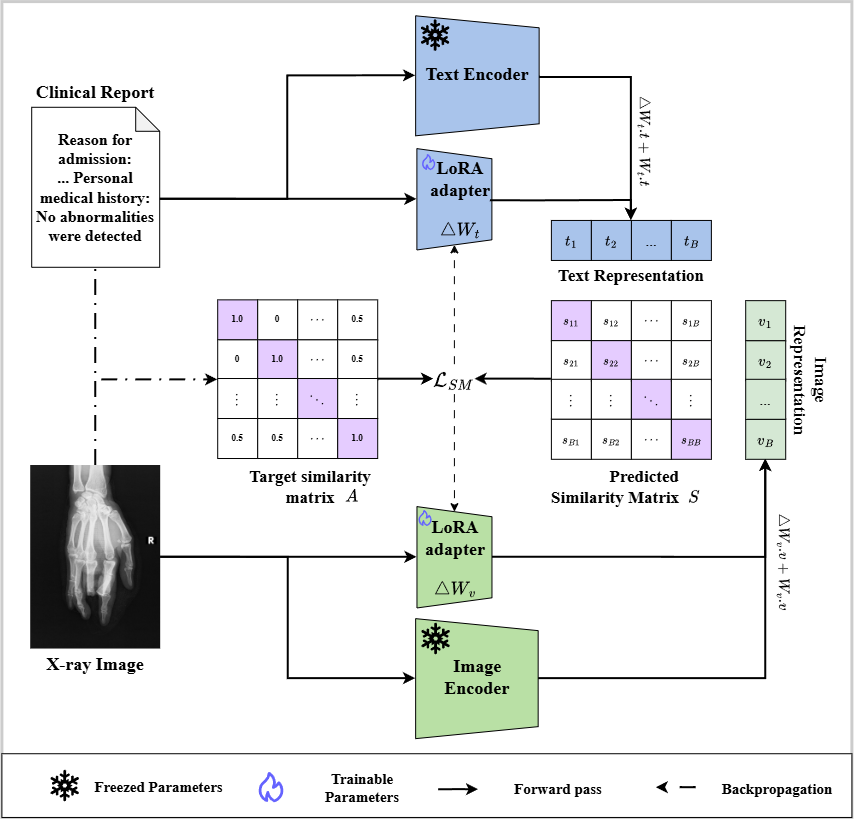
\includegraphics[width=\columnwidth]{phase1.png}
\caption{Phase 1: class-aware image--text alignment with soft matching targets. The pretrained encoder weights remain frozen while the LoRA adapters are optimized.}
\label{fig:phase1}
\end{figure}

\subsection{Phase 2: Bidirectional Fusion and Classification}
Phase~2 uses the encoders' native token sequences (Fig.~\ref{fig:phase2}). Tokens are layer-normalized and projected to 512 dimensions, with additional normalization of global tokens. Each global token queries the other modality's local tokens through eight-head attention. Reusing the token notation for these transformed features, the residual summaries are
\begin{equation}
\begin{aligned}
h_I&=\operatorname{LN}\big(v_0+\operatorname{Drop}(\operatorname{MHA}(v_0,T_\ell,T_\ell;M_T))\big),\\
h_T&=\operatorname{LN}\big(t_0+\operatorname{Drop}(\operatorname{MHA}(t_0,V_\ell,V_\ell))\big),
\end{aligned}
\label{eq:fusion}
\end{equation}
where $M_T$ masks text padding. Thus, image features condition the selection of textual features and history conditions the selection of visual features. The summaries pass through a $1024\to512\to512$ MLP with GELU and dropout, followed by a linear classifier:
\begin{equation}
z=\operatorname{LN}(\operatorname{MLP}([h_I;h_T])),\quad
p=\operatorname{softmax}(W_cz+b_c).
\end{equation}

The supervised objective combines effective-number class weighting~\cite{Cui2019ClassBalanced} with label smoothing. For class $c$ with $n_c$ training examples, define its effective number and inverse weight as
\begin{equation}
E_c=\frac{1-\beta^{n_c}}{1-\beta},\qquad a_c=E_c^{-1},\quad\beta=0.999.
\end{equation}
The normalized weight is clipped at five:
\begin{equation}
w_c=\min\left(\frac{Ka_c}{\sum_j a_j},5\right).
\end{equation}
Label smoothing regularizes the target distribution:
\begin{equation}
u_{ic}=(1-\epsilon)\ind[y_i=c]+\frac{\epsilon}{K},\qquad\epsilon=0.1.
\end{equation}
The resulting weighted cross-entropy is
\begin{equation}
\mathcal L_{\mathrm{cls}}=-\frac{\sum_i\sum_c w_cu_{ic}\log p_{ic}}{\sum_i w_{y_i}},
\label{eq:loss}
\end{equation}
where $p_{ic}$ is the predicted class probability. Weights use training counts only and apply to all smoothed target terms. Phase~2 updates adapters, fusion, and the classifier while pretrained encoder weights remain frozen. Individual effects of weighting and smoothing require separate ablations.

\begin{figure}[t]
\centering
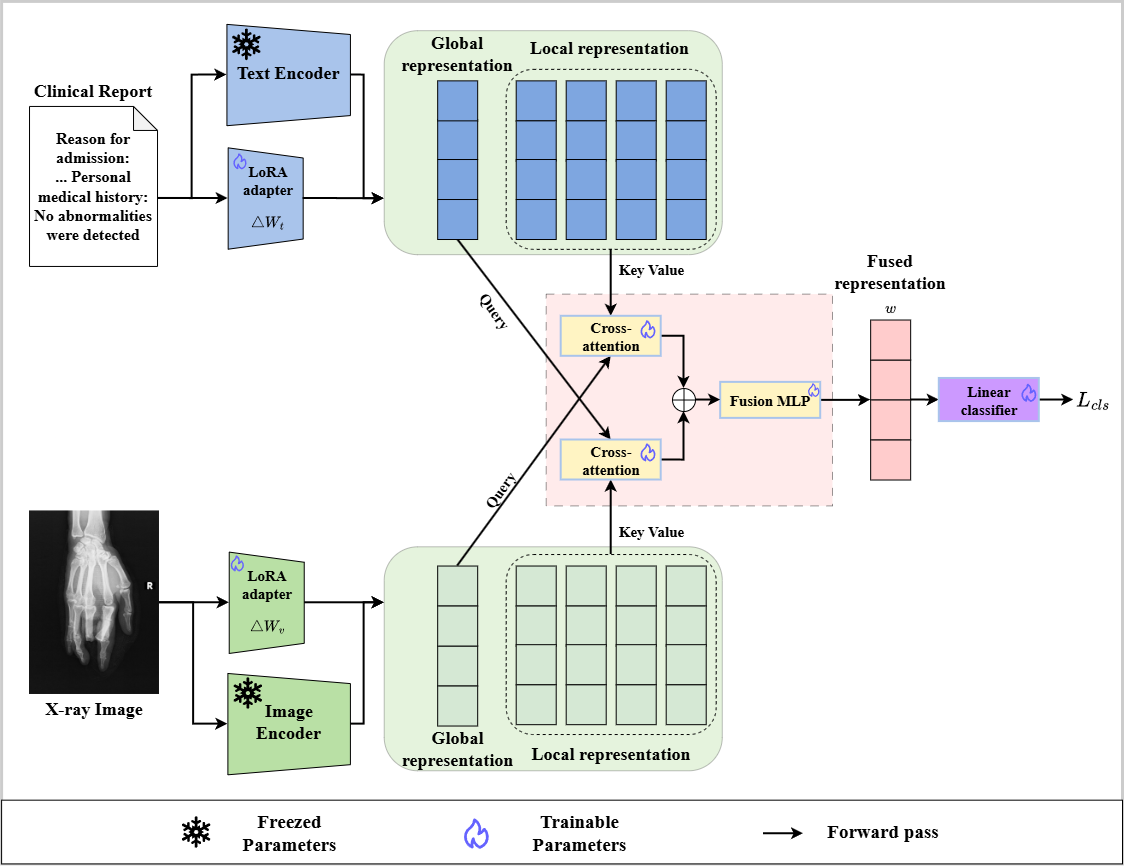
\includegraphics[width=\columnwidth]{phase2.png}
\caption{Phase 2: bidirectional global-to-local fusion and classification, initialized with the Phase-1 adapters. The selected model supplies fixed-weight online inference.}
\label{fig:phase2}
\end{figure}

\subsection{Integrated Gradients Attribution}
Integrated Gradients (IG)~\cite{Sundararajan2017IntegratedGradients} attributes the original predicted-class logit $F_{\hat y}$ to input components relative to reference $u^0$:
\begin{equation}
\operatorname{IG}_j(u,u^0)=(u_j-u_j^0)\int_0^1
\frac{\partial F_{\hat y}(u^0+\lambda(u-u^0))}{\partial u_j}\,d\lambda.
\end{equation}
We hold the other modality fixed. The image reference is the zero tensor in normalized image space, whereas the text reference replaces content embeddings with padding embeddings while preserving special tokens and masks. Attribution-ranked deletion measures changes in the original predicted-class probability. Deletion AUC integrates this probability over the fraction removed. These interventions characterize input dependence under the specified references without establishing lesion localization or clinical correctness.


\section{Experiments}
\subsection{Experimental Setup}
Each reported classification result aggregates independent training runs with seeds 42, 123, and 456. Table~\ref{tab:setup} specifies the XBone-Net recipe. Checkpoints minimize validation loss in Phase~1 and maximize validation Macro-F1 in Phase~2. Images use BiomedCLIP's native RGB resize, center crop to $224\times224$, and normalization. Text uses its tokenizer with maximum length 256. No additional lesion crops or image branches are used.

\begin{table}[t]
\caption{XBone-Net training configuration. Epoch counts are maxima, and patience is in validation evaluations.}
\label{tab:setup}
\centering\footnotesize
\begin{tabularx}{\columnwidth}{@{}lY@{}}
\toprule
Setting & Value \\
\midrule
Hardware / precision & NVIDIA RTX 5060 Ti / BF16 \\
Optimizer / schedule & AdamW / cosine decay \\
Batch / accumulation & 16 / 1 \\
Weight decay & $10^{-4}$ \\
Phase 1 & 30 epochs, LR $5\times10^{-5}$, patience 3 \\
Phase 2 & 50 epochs, LR $10^{-4}$, patience 5 \\
LoRA & Rank 16, scaling 32, dropout 0.1 \\
Fusion & 512 dimensions, 8 heads, dropout 0.1 \\
Loss & $\rho=0.5$, $\beta=0.999$, $\epsilon=0.1$, weight cap 5 \\
\bottomrule
\end{tabularx}
\end{table}

\subsection{Datasets}
\textbf{CTCH} contains 3,249 radiograph--history pairs in 22 classes, including normal findings and fracture categories, from a single orthopedic hospital in Ho Chi Minh City. The patient-level split comprises 2,265 training, 315 validation, and 669 test cases with no shared patient keys. Text combines the reason for admission, disease history, and personal medical history, translated from Vietnamese into English. Explicit diagnostic-label and radiographic-finding fields are excluded. Prior diagnoses can nevertheless occur within history, and terminology may be affected by translation. The data are de-identified and used under a research confidentiality agreement. Source clinical records are not publicly released.

\textbf{BTXRD}~\cite{Yao2025} contains 3,746 images in our ten-class formulation of normal findings and bone-tumor categories, with a 2,621/375/750 image-level split. Stable patient identifiers are unavailable for this partition. Text is generated from metadata conditioned on disease groups. Consequently, this experiment evaluates the recipe with label-correlated synthetic text. It does not independently establish the benefit of real clinical histories.

Table~\ref{tab:datasets} characterizes imbalance in the test cohorts. The largest classes contain 32.6\% of CTCH cases and 48.8\% of BTXRD images, whereas the smallest contain only six and nine cases. We therefore report Macro-F1 and balanced accuracy alongside accuracy. Macro-F1 averages class F1 scores, whereas balanced accuracy averages class recalls. Classification results are reported as mean $\pm$ sample SD across three training seeds on the same split.

\begin{table}[t]
\caption{Dataset partitions and test-class support. Ratio is the largest divided by the smallest test-class count.}
\label{tab:datasets}
\centering\footnotesize
\begin{tabular}{@{}lcc@{}}
\toprule
Property & CTCH & BTXRD \\
\midrule
Classes & 22 & 10 \\
Train / validation / test & 2265 / 315 / 669 & 2621 / 375 / 750 \\
Split unit & Patient & Image \\
Text source & Clinical history & Synthetic metadata \\
Test count: min / median / max & 6 / 18.5 / 218 & 9 / 35.5 / 366 \\
Max/min ratio & $36.3\times$ & $40.7\times$ \\
\bottomrule
\end{tabular}
\end{table}

\subsection{Multimodal Image Classification}
Table~\ref{tab:classification} compares six locally trained baselines: ResNet-50 and DenseNet-121 use images only, whereas CLIP, MedCLIP, PubMedCLIP~\cite{PubMedCLIP}, and BiomedCLIP use image--text pairs with full encoder tuning and global feature concatenation. Fully tuned BiomedCLIP uses learning rate $2\times10^{-5}$. These comparisons evaluate complete adaptation recipes rather than a controlled backbone substitution. The CTCH Image-only variant additionally removes history, Phase~1, and cross-modal fusion.

\begin{table*}[t]
\caption{Classification performance (\%, mean $\pm$ SD across three seeds). Best results are bold, and second-best results are underlined. The proposed configurations are separated from the six baselines and their names are bold.}
\label{tab:classification}
\centering\footnotesize
\setlength{\tabcolsep}{6pt}
\begin{tabular*}{\textwidth}{@{\extracolsep{\fill}}lcccccc@{}}
\toprule
Method & \multicolumn{3}{c}{CTCH (22 classes, $n=669$)} & \multicolumn{3}{c}{BTXRD (10 classes, $n=750$)} \\
\cmidrule(lr){2-4}\cmidrule(l){5-7}
 & Accuracy & Balanced acc. & Macro-F1 & Accuracy & Balanced acc. & Macro-F1 \\
\midrule
ResNet-50 & $49.83\pm0.77$ & $41.80\pm0.46$ & $41.54\pm0.20$ & $60.67\pm1.33$ & $31.80\pm1.31$ & $32.85\pm0.96$ \\
DenseNet-121 & $48.18\pm0.38$ & $49.20\pm4.65$ & $43.60\pm2.42$ & $63.20\pm0.13$ & $36.94\pm1.50$ & $37.18\pm1.73$ \\
CLIP & $58.74\pm2.09$ & $\mathbf{62.17\pm3.59}$ & $\underline{56.33\pm0.90}$ & $80.36\pm2.73$ & $59.57\pm1.60$ & $57.87\pm2.52$ \\
MedCLIP & $56.00\pm3.96$ & $57.23\pm1.77$ & $51.61\pm2.24$ & $82.09\pm1.47$ & $\mathbf{61.27\pm2.38}$ & $\underline{60.57\pm1.53}$ \\
PubMedCLIP & $55.21\pm2.34$ & $55.89\pm6.14$ & $52.03\pm2.64$ & $78.84\pm2.85$ & $60.89\pm3.42$ & $57.23\pm5.77$ \\
BiomedCLIP & $\underline{59.69\pm2.53}$ & $\underline{60.23\pm2.34}$ & $55.40\pm0.80$ & $\mathbf{83.11\pm0.28}$ & $60.62\pm2.54$ & $59.94\pm1.24$ \\
\midrule
\textbf{XBone-Net Image-only (ours)} & $44.39\pm6.89$ & $48.43\pm1.36$ & $38.13\pm5.51$ & $64.23\pm1.54$ & $32.67\pm1.69$ & $40.21\pm2.57$ \\
\textbf{XBone-Net (ours)} & $\mathbf{61.83\pm2.03}$ & $59.35\pm1.34$ & $\mathbf{57.27\pm1.93}$ & $\underline{83.02\pm0.98}$ & $\underline{61.15\pm1.40}$ & $\mathbf{62.40\pm1.18}$ \\
\bottomrule
\end{tabular*}
\end{table*}


On CTCH, XBone-Net yields the highest observed accuracy and Macro-F1, with Macro-F1 gains of 1.87 percentage points over BiomedCLIP and 0.94 over CLIP. CLIP instead has higher balanced accuracy (62.17\% versus 59.35\%). On BTXRD, XBone-Net has the highest observed Macro-F1 (62.40\%), while BiomedCLIP and MedCLIP lead in accuracy and balanced accuracy, respectively. The gain is therefore metric dependent. The sizable gap between accuracy and Macro-F1 also indicates uneven class performance. Higher aggregate Macro-F1 does not demonstrate improved recall for every rare diagnosis.

The CTCH resource profile in Table~\ref{tab:cost} quantifies the practical trade-off. XBone-Net updates 8.45M parameters, approximately 95.7\% fewer than full tuning, and lowers mean peak allocated training memory from 3816.8 to 1455.0 MiB. This reduces memory demand during local adaptation. However, training takes 2.50 times as long and measured inference latency rises from 13.77 to 16.17 ms. Parameter efficiency therefore concerns the optimized state and training memory, rather than faster execution.

\begin{table}[t]
\caption{CTCH resource trade-off against full BiomedCLIP tuning. Training time and peak allocated memory are mean $\pm$ SD across three seeds, whereas inference is profiled at seed 42.}
\label{tab:cost}
\centering\footnotesize
\begin{tabular}{@{}lcc@{}}
\toprule
Measure & BiomedCLIP & \textbf{XBone-Net (ours)} \\
\midrule
Training model parameters (M) & 196.44 & 204.35 \\
Trainable parameters (M) & 196.44 & 8.45 \\
Trainable fraction (\%) & 100.00 & 4.13 \\
Training time (GPU-hours) & $0.3411\pm0.0800$ & $0.8542\pm0.0925$ \\
Peak allocated memory (MiB) & $3816.8\pm0.0$ & $1455.0\pm43.0$ \\
\midrule
Inference parameters (M) & 196.44 & 199.34 \\
GFLOPs & 81.03 & 82.32 \\
Latency (ms) & 13.77 & 16.17 \\
Throughput (samples/s) & 75.6 & 64.1 \\
\bottomrule
\end{tabular}
\end{table}

Training costs include both phases and their validation/checkpoint operations, excluding model loading and data-loader construction. Inference uses merged LoRA weights, BF16, and batch size one on the same GPU: 20 inputs, each with ten warm-up and ten timed forwards. Latency excludes data loading and host-to-device transfer and therefore does not measure end-to-end clinical workflow time.

\subsection{Ablation Study}
We compare internal CTCH variants on the same 669 test cases and three seeds. Phase~2 only omits alignment, while Concatenation replaces bidirectional cross-attention with global concatenation. Table~\ref{tab:ablation} isolates these architecture comparisons, while the Image-only control is reported in Table~\ref{tab:classification}.

\begin{table}[t]
\caption{CTCH architecture ablations (\%, mean $\pm$ SD across three seeds). Best results are bold, and second-best results are underlined. The Image-only control is reported in Table~\ref{tab:classification}.}
\label{tab:ablation}
\centering\footnotesize
\setlength{\tabcolsep}{3.5pt}
\begin{tabular}{@{}lccc@{}}
\toprule
Configuration & Accuracy & Balanced acc. & Macro-F1 \\
\midrule
\textbf{XBone-Net (ours)} & $\mathbf{61.83\pm2.03}$ & $\underline{59.35\pm1.34}$ & $\mathbf{57.27\pm1.93}$ \\
Phase 2 only & $\underline{60.04\pm0.85}$ & $55.52\pm3.41$ & $\underline{54.97\pm1.84}$ \\
Concatenation & $58.25\pm0.38$ & $\mathbf{59.83\pm2.68}$ & $54.77\pm1.62$ \\
\bottomrule
\end{tabular}
\end{table}


Removing Phase~1 lowers mean Macro-F1 by 2.30 percentage points, and substituting concatenation lowers it by 2.50. Concatenation retains slightly higher balanced accuracy. These observations motivate alignment and conditional fusion, but the experiment does not establish their independent benefit across other splits or institutions. The 19.14-point Macro-F1 difference between full and Image-only configurations reflects the combined change in text access, alignment, and fusion. Isolated loss, sampler, and history-replacement experiments are needed to identify which mechanisms drive the difference.

\subsection{Modality Contribution and Input Dependence}
We analyze all 669 CTCH test cases at seed 42, including incorrect predictions, using 24 IG interpolation points. Interventions remove $16\times16$ image patches or text content units while fixing the other modality. Each model retains its original predicted class as the target, with 16 random deletion orders per case.

Figure~\ref{fig:ig} shows lower targeted than random deletion AUC for images (0.2997 versus 0.3405) and text (0.2811 versus 0.3588). Whole-source replacement reduces predicted-class probability by 0.3187 for images and 0.2725 for text on average. These results indicate dependence on both inputs under the specified interventions. They neither establish region--word correspondence nor quantify cross-modal interaction. Different intervention units and references also preclude directly ranking the modalities by their deletion gaps.

XBone-Net has higher image insertion AUC than Image-only (0.4023 versus 0.2517), but also higher deletion AUC (0.2997 versus 0.1541). Because these values depend on model confidence and target class, they do not establish superior explanation quality. Lesion annotations, controlled history perturbations, and clinician review remain necessary to assess clinical plausibility.

\begin{figure*}[t]
\centering
\begin{tikzpicture}
\begin{groupplot}[
group style={group size=2 by 1,horizontal sep=13mm},
width=.46\textwidth,height=38mm,
xmin=0,xmax=1,ymin=0,ymax=.65,
xtick={0,.5,1},ytick={0,.2,.4,.6},
xlabel={Fraction removed},
axis lines=left,axis line style={black!60},
ymajorgrids,grid style={black!12},
tick label style={font=\footnotesize},
label style={font=\footnotesize},title style={font=\small\bfseries},
legend style={font=\scriptsize,draw=none,fill=none,at={(.98,.98)},anchor=north east},
]
\nextgroupplot[title={(a) Image patches},ylabel={Predicted-class probability}]
\addplot[color=red!70!black,line width=1.1pt] table[x=fraction,y=targeted]{ig_image.dat};
\addplot[color=blue!65!black,line width=1pt,dashed] table[x=fraction,y=random]{ig_image.dat};
\node[anchor=south west,font=\footnotesize,align=left] at (axis cs:.035,.025) {AUC gap: 0.0409};
\nextgroupplot[title={(b) Clinical-text units}]
\addplot[color=red!70!black,line width=1.1pt] table[x=fraction,y=targeted]{ig_text.dat};
\addlegendentry{IG-targeted deletion}
\addplot[color=blue!65!black,line width=1pt,dashed] table[x=fraction,y=random]{ig_text.dat};
\addlegendentry{Random deletion}
\node[anchor=south west,font=\footnotesize] at (axis cs:.035,.025) {AUC gap: 0.0777};
\end{groupplot}
\end{tikzpicture}

\caption{IG-guided deletion on all 669 CTCH test cases (seed 42). Curves average original predicted-class probabilities and compare IG order with 16 random orders per case. AUC gaps are random minus targeted deletion AUC. Each intervention fixes the other modality.}
\label{fig:ig}
\end{figure*}


Figure~\ref{fig:ig_case} illustrates CTCH case 3563, correctly classified as finger fracture with probability 0.5005. The author-selected example displays image relevance and signed word contributions for the same prediction. Relevance also extends beyond bone structures, illustrating the distinction between input sensitivity and validated lesion localization.

\begin{figure*}[t]
\centering
\begingroup
\centering
{\small\textbf{CTCH case 3563: Finger fracture} $\vert$ Prediction: Finger fracture (50.0\%)}\par\smallskip
\begin{minipage}[t]{0.185\linewidth}
\centering\vspace{0pt}
{\footnotesize\textbf{(a) Radiograph}}\par\smallskip
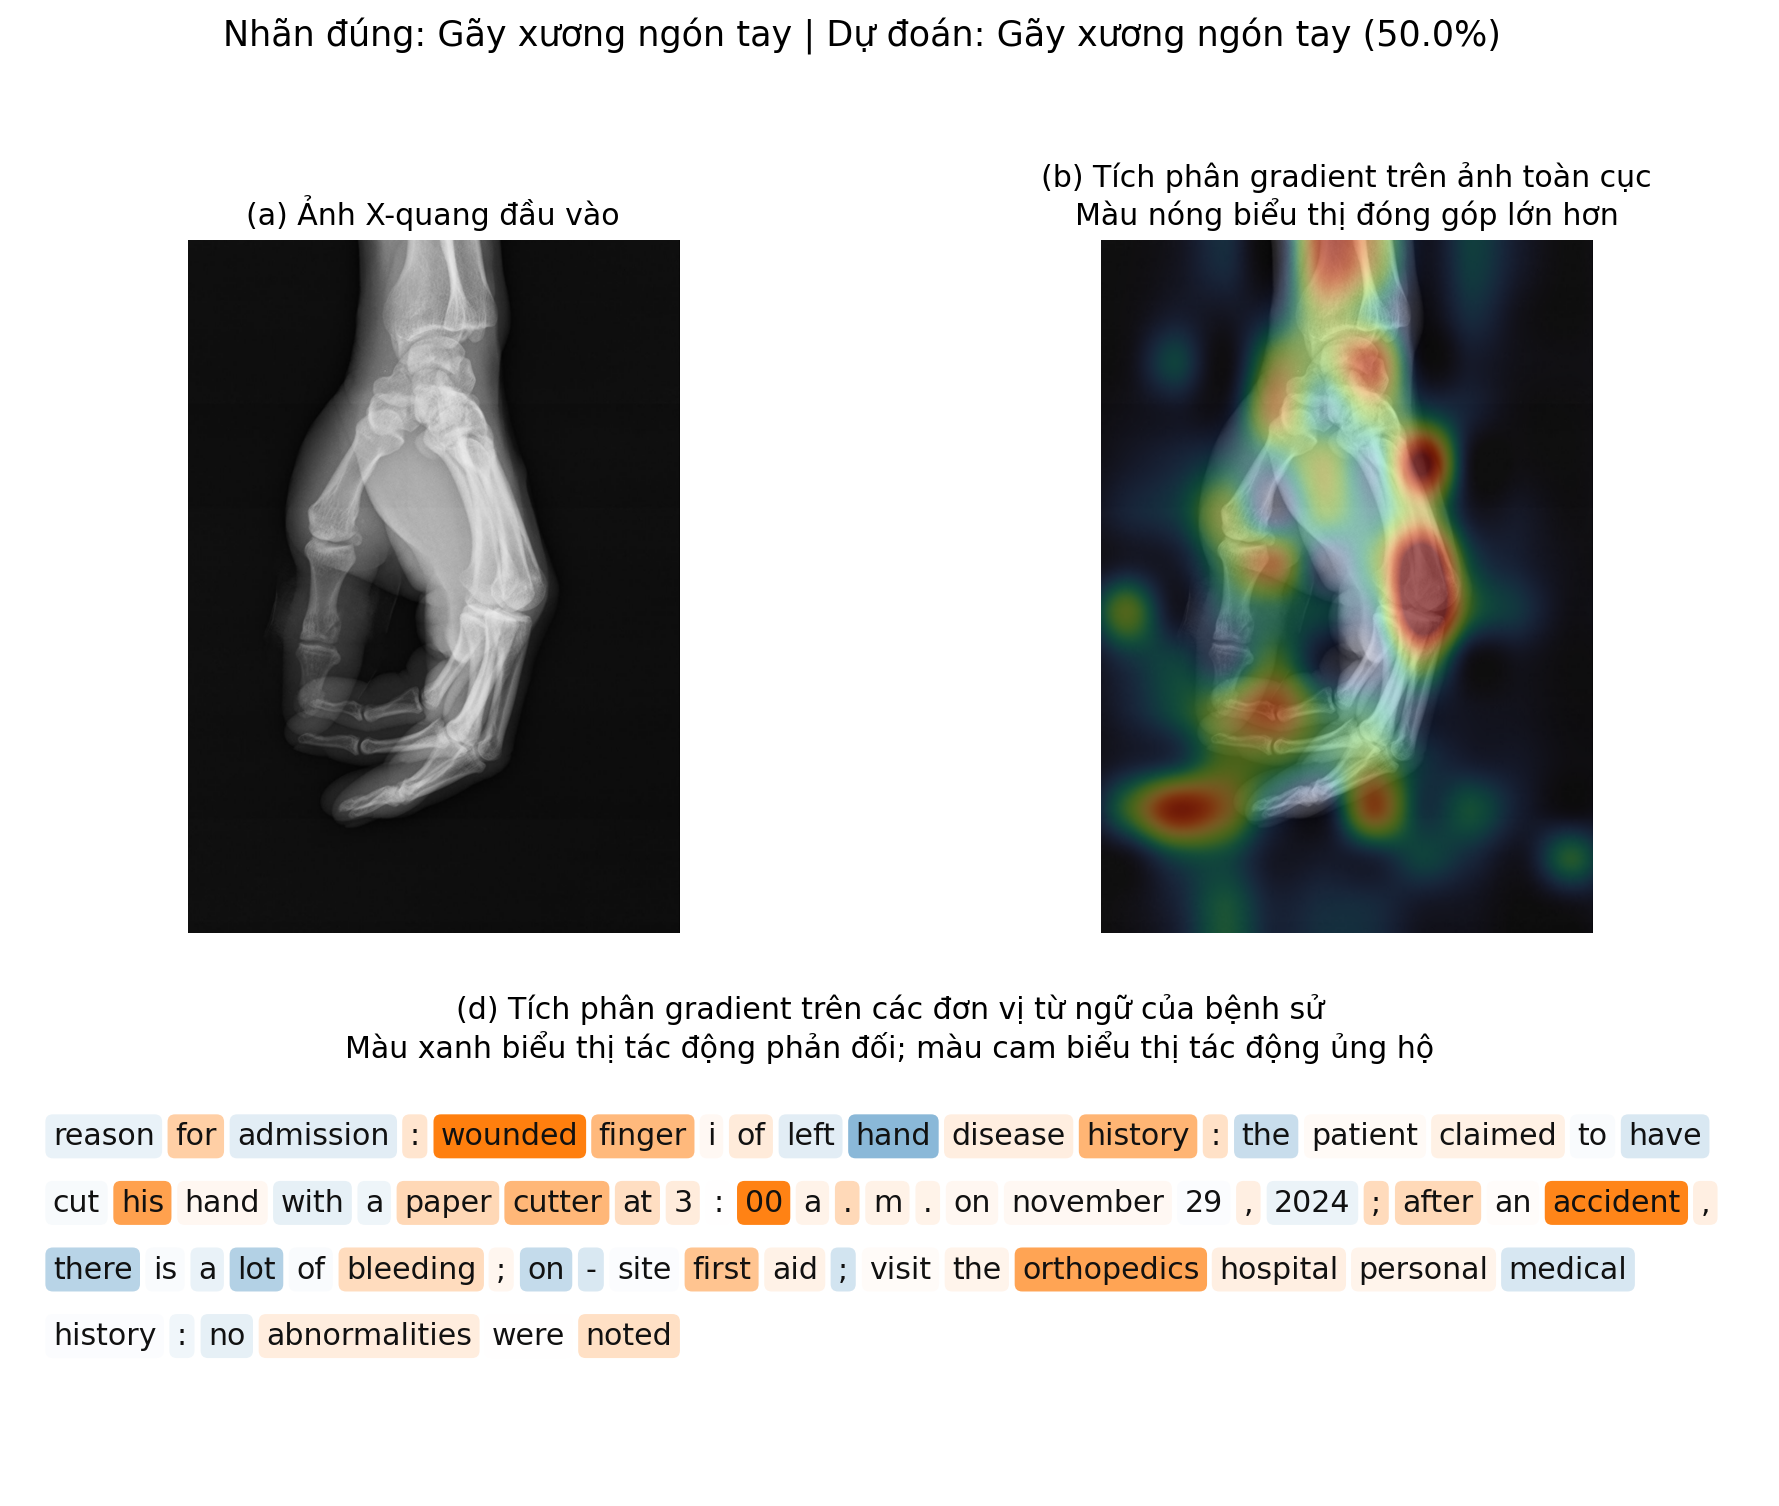
\includegraphics[trim={75.19591bp 229.18752bp 439.57607bp 95.99477bp},clip,width=\linewidth]{ig_case_source.png}
\end{minipage}\hfill
\begin{minipage}[t]{0.185\linewidth}
\centering\vspace{0pt}
{\footnotesize\textbf{(b) Image IG}}\par\smallskip
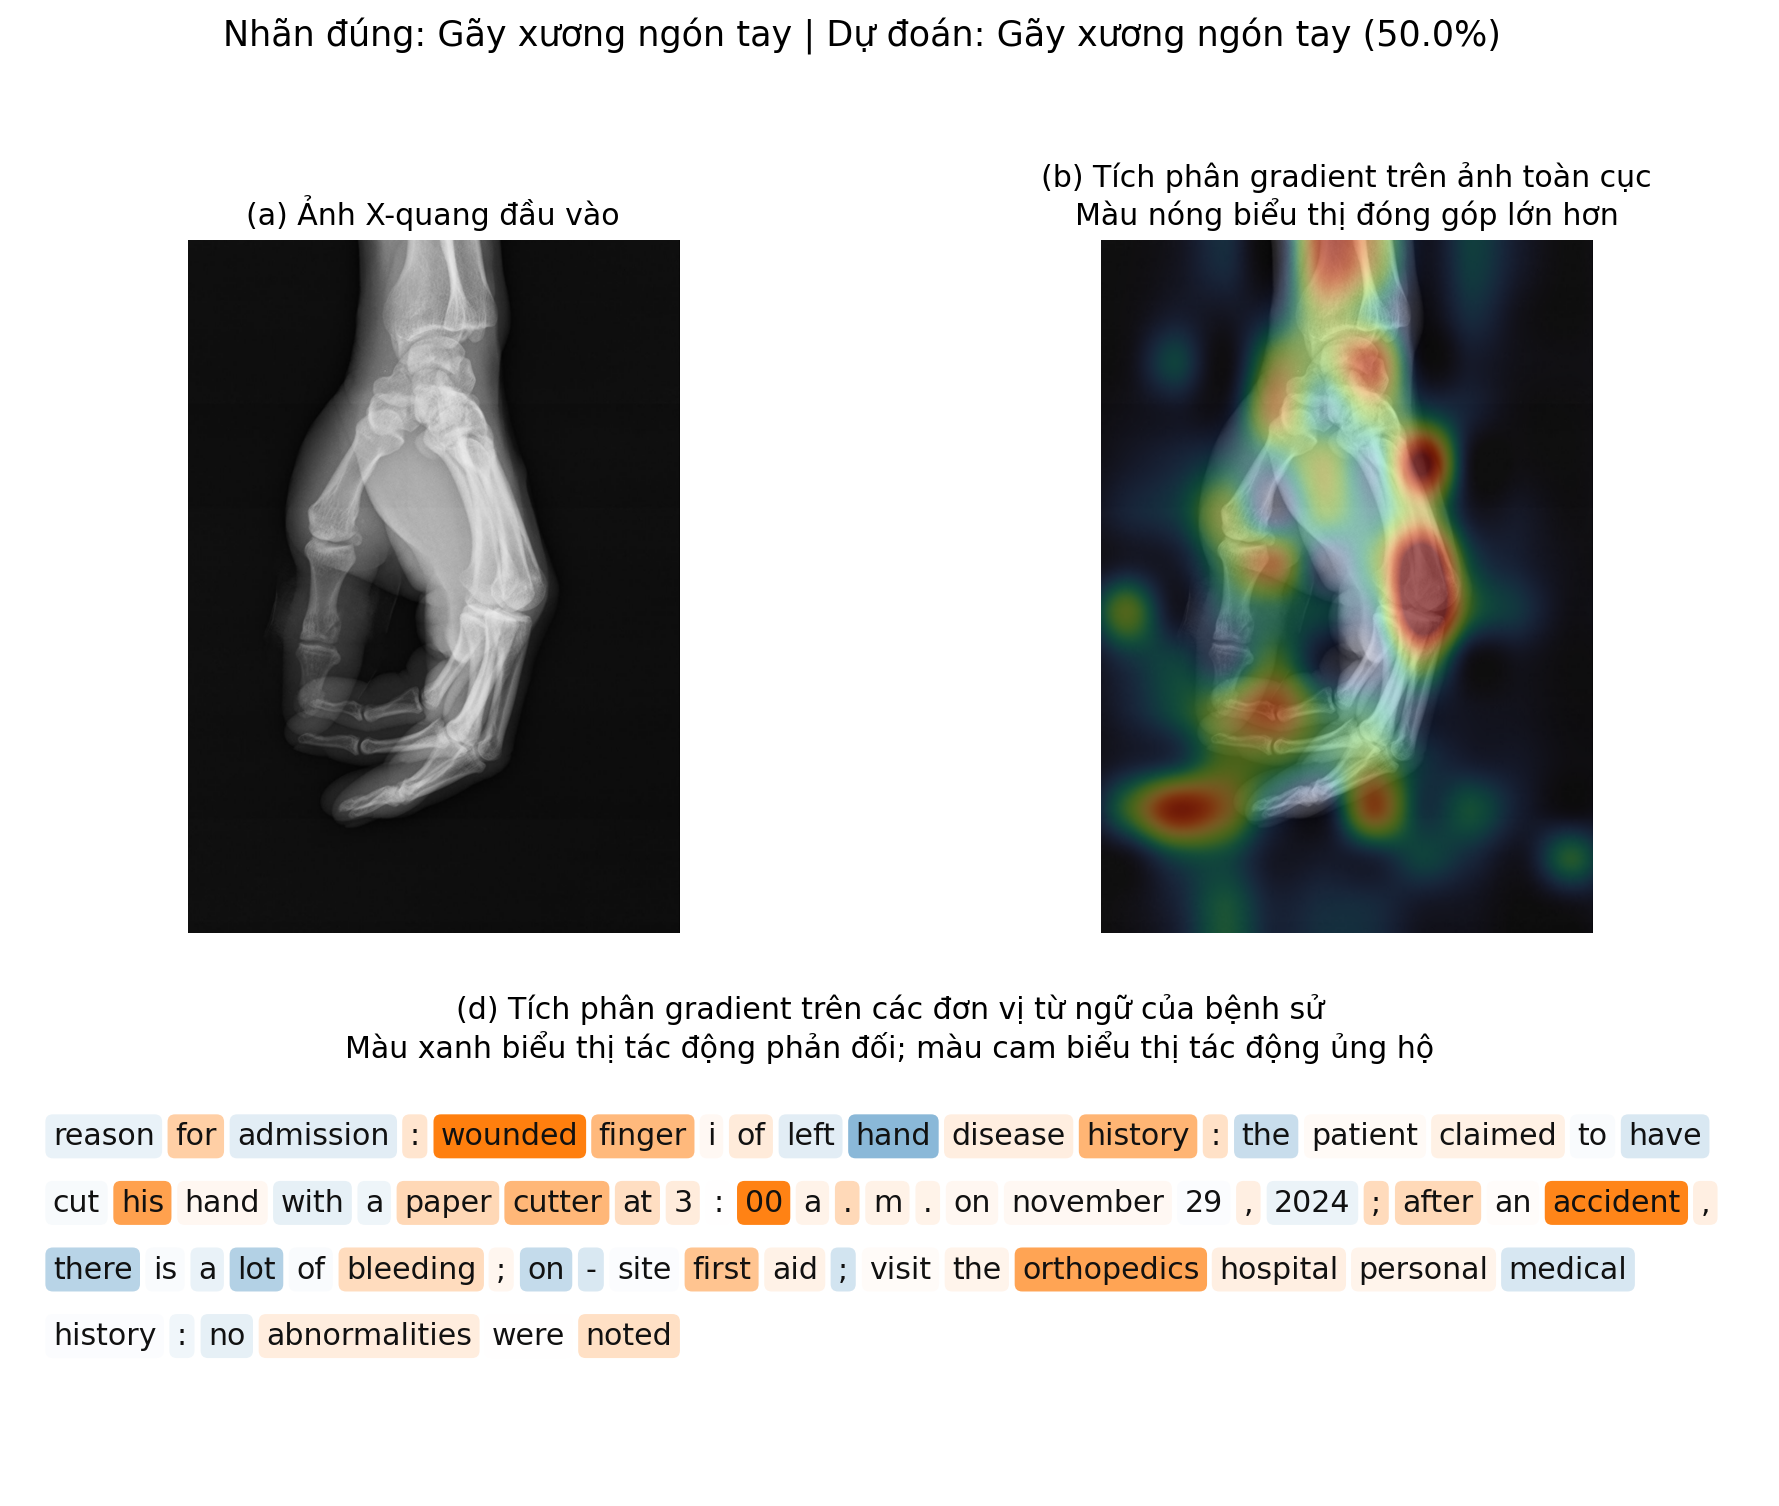
\includegraphics[trim={440.37602bp 229.18752bp 74.39595bp 95.99477bp},clip,width=\linewidth]{ig_case_source.png}
\end{minipage}\hfill
\begin{minipage}[t]{0.59\linewidth}
\raggedright\vspace{0pt}
{\footnotesize\textbf{(c) Clinical-text IG}}\par\smallskip
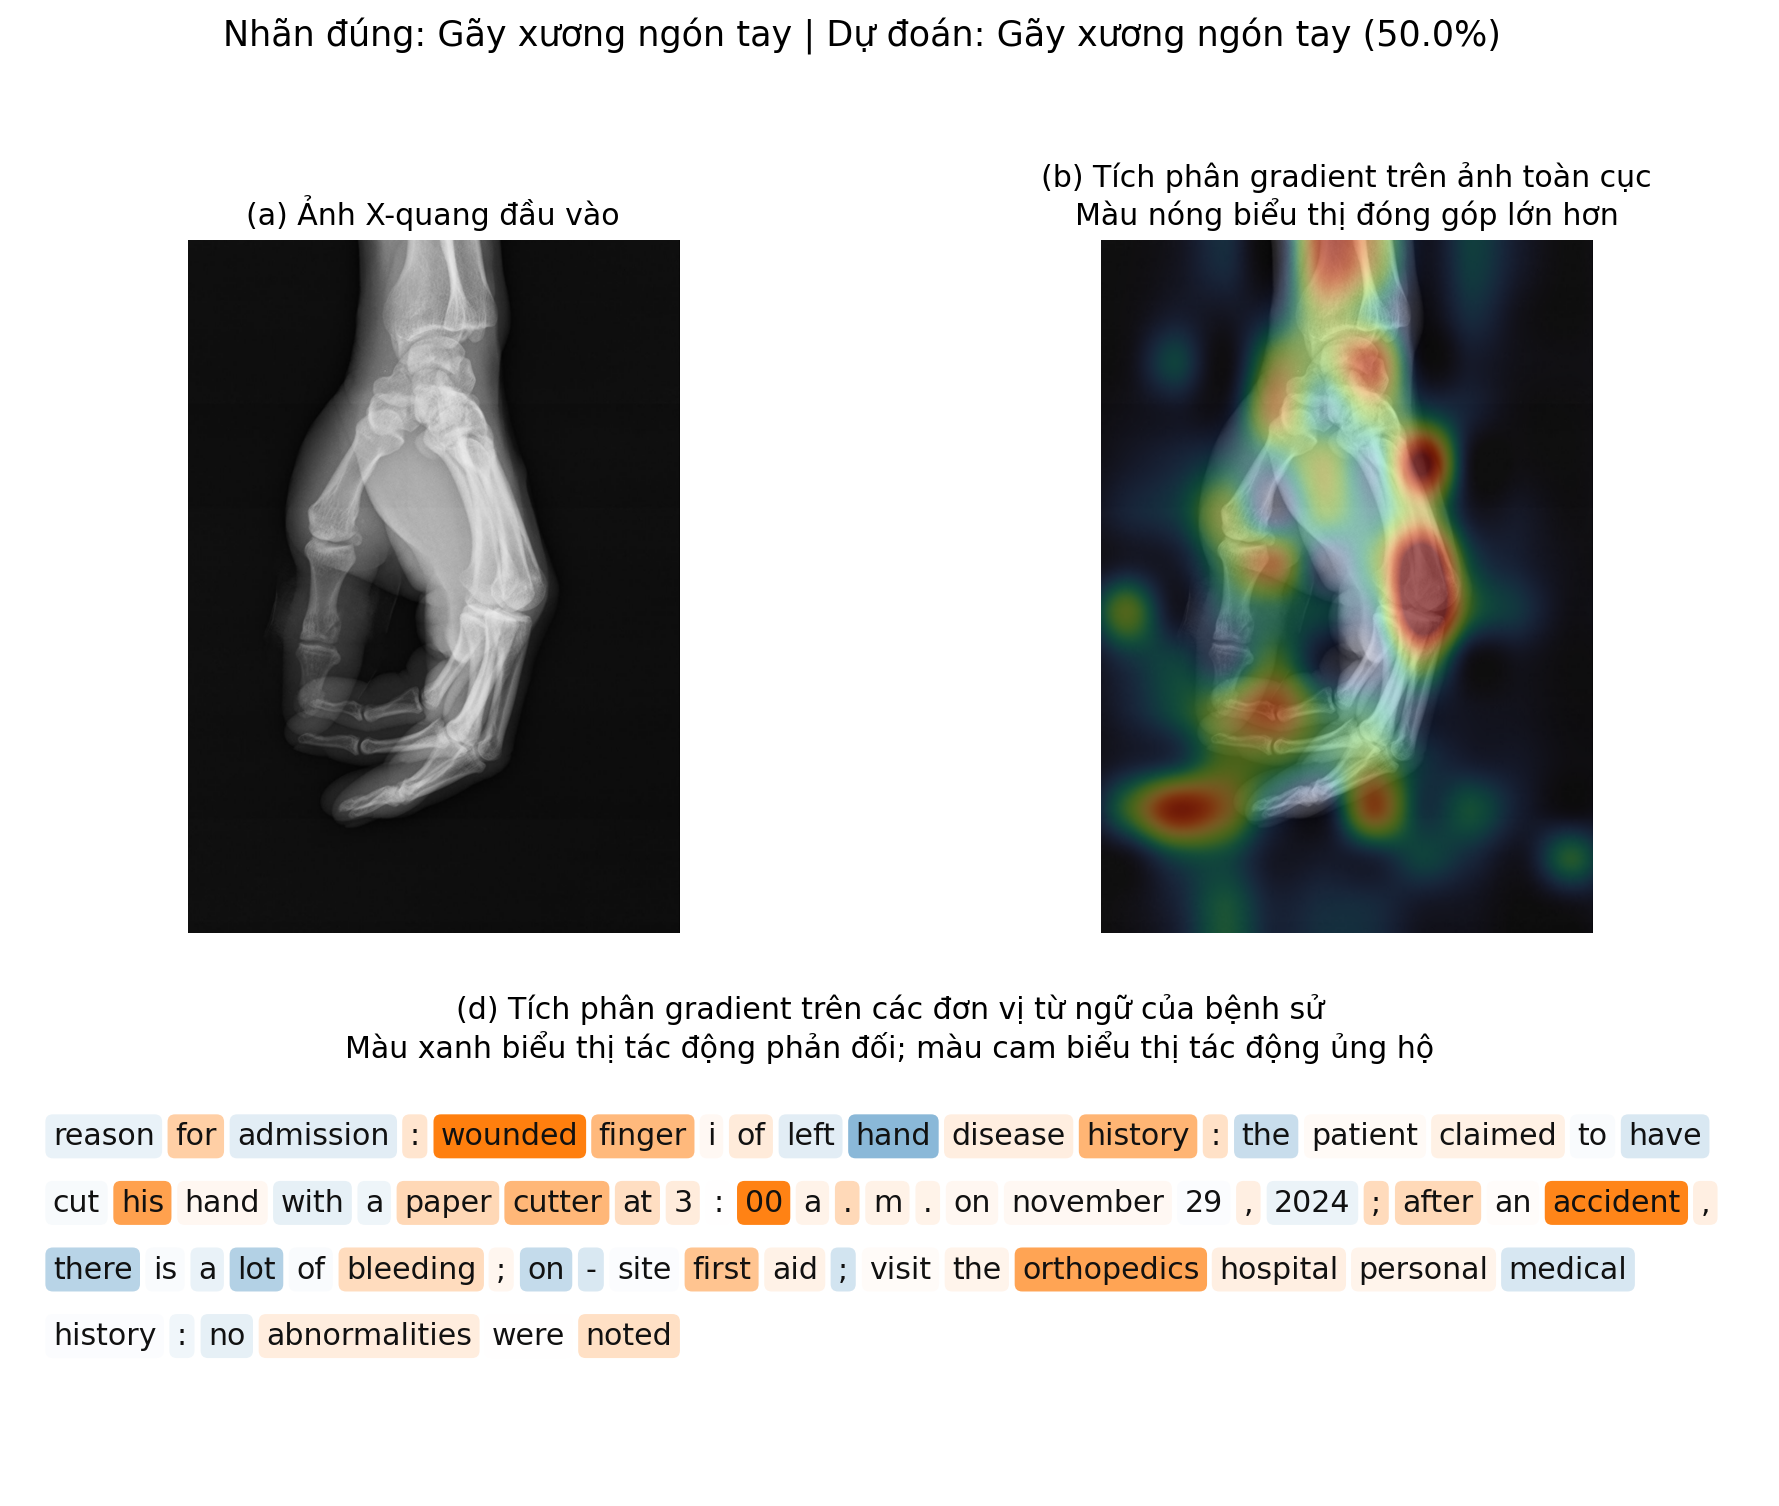
\includegraphics[trim={17.19906bp 137.99249bp 373.57966bp 444.77578bp},clip,width=0.926097\linewidth]{ig_case_source.png}\\[-1pt]
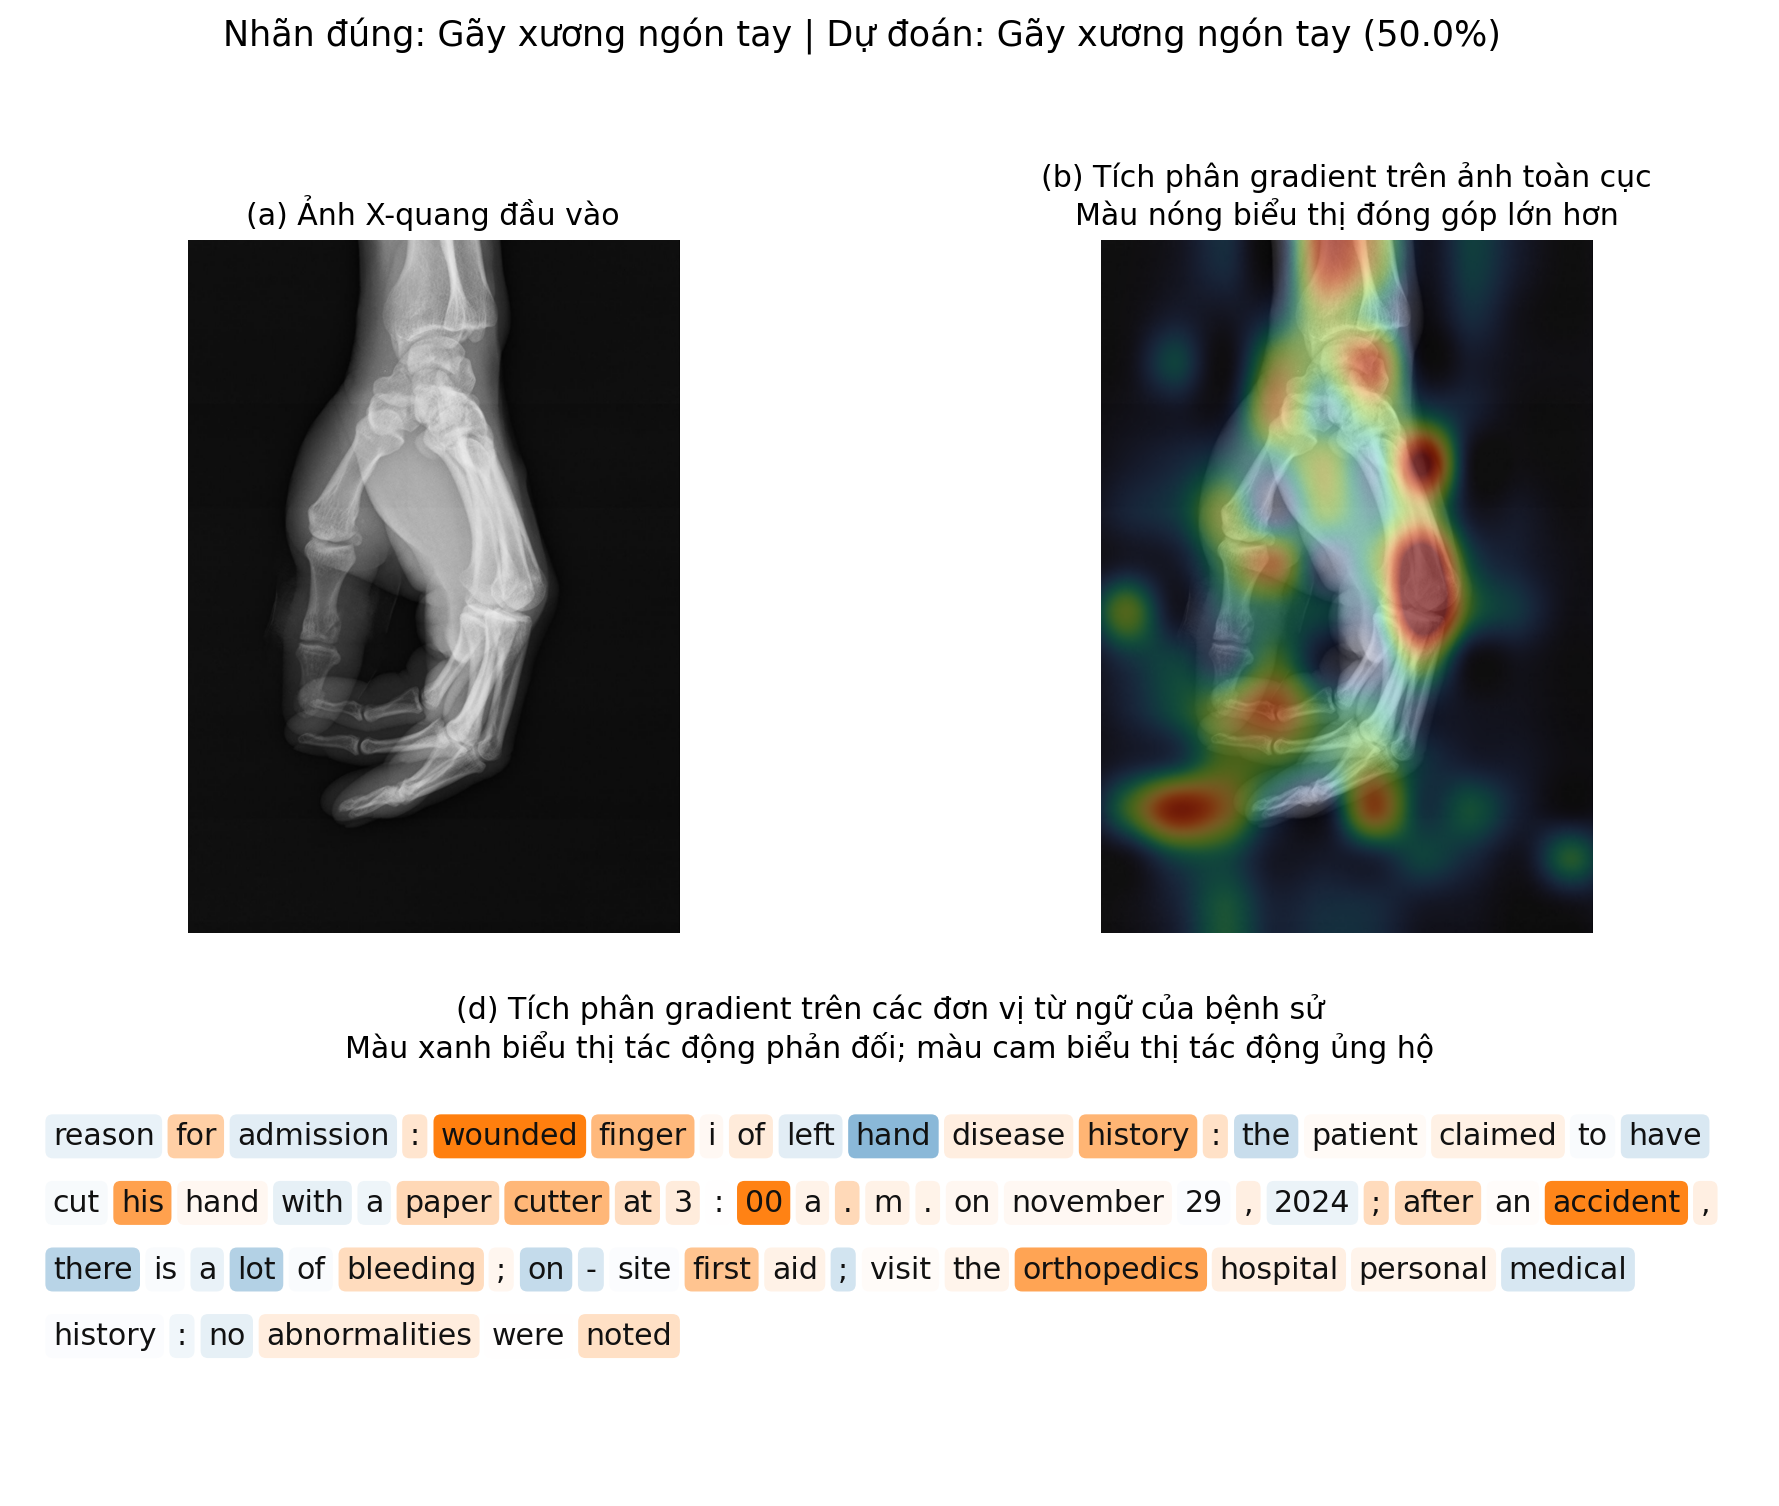
\includegraphics[trim={338.38158bp 137.99249bp 26.79854bp 444.77578bp},clip,width=1.000000\linewidth]{ig_case_source.png}\\[-1pt]
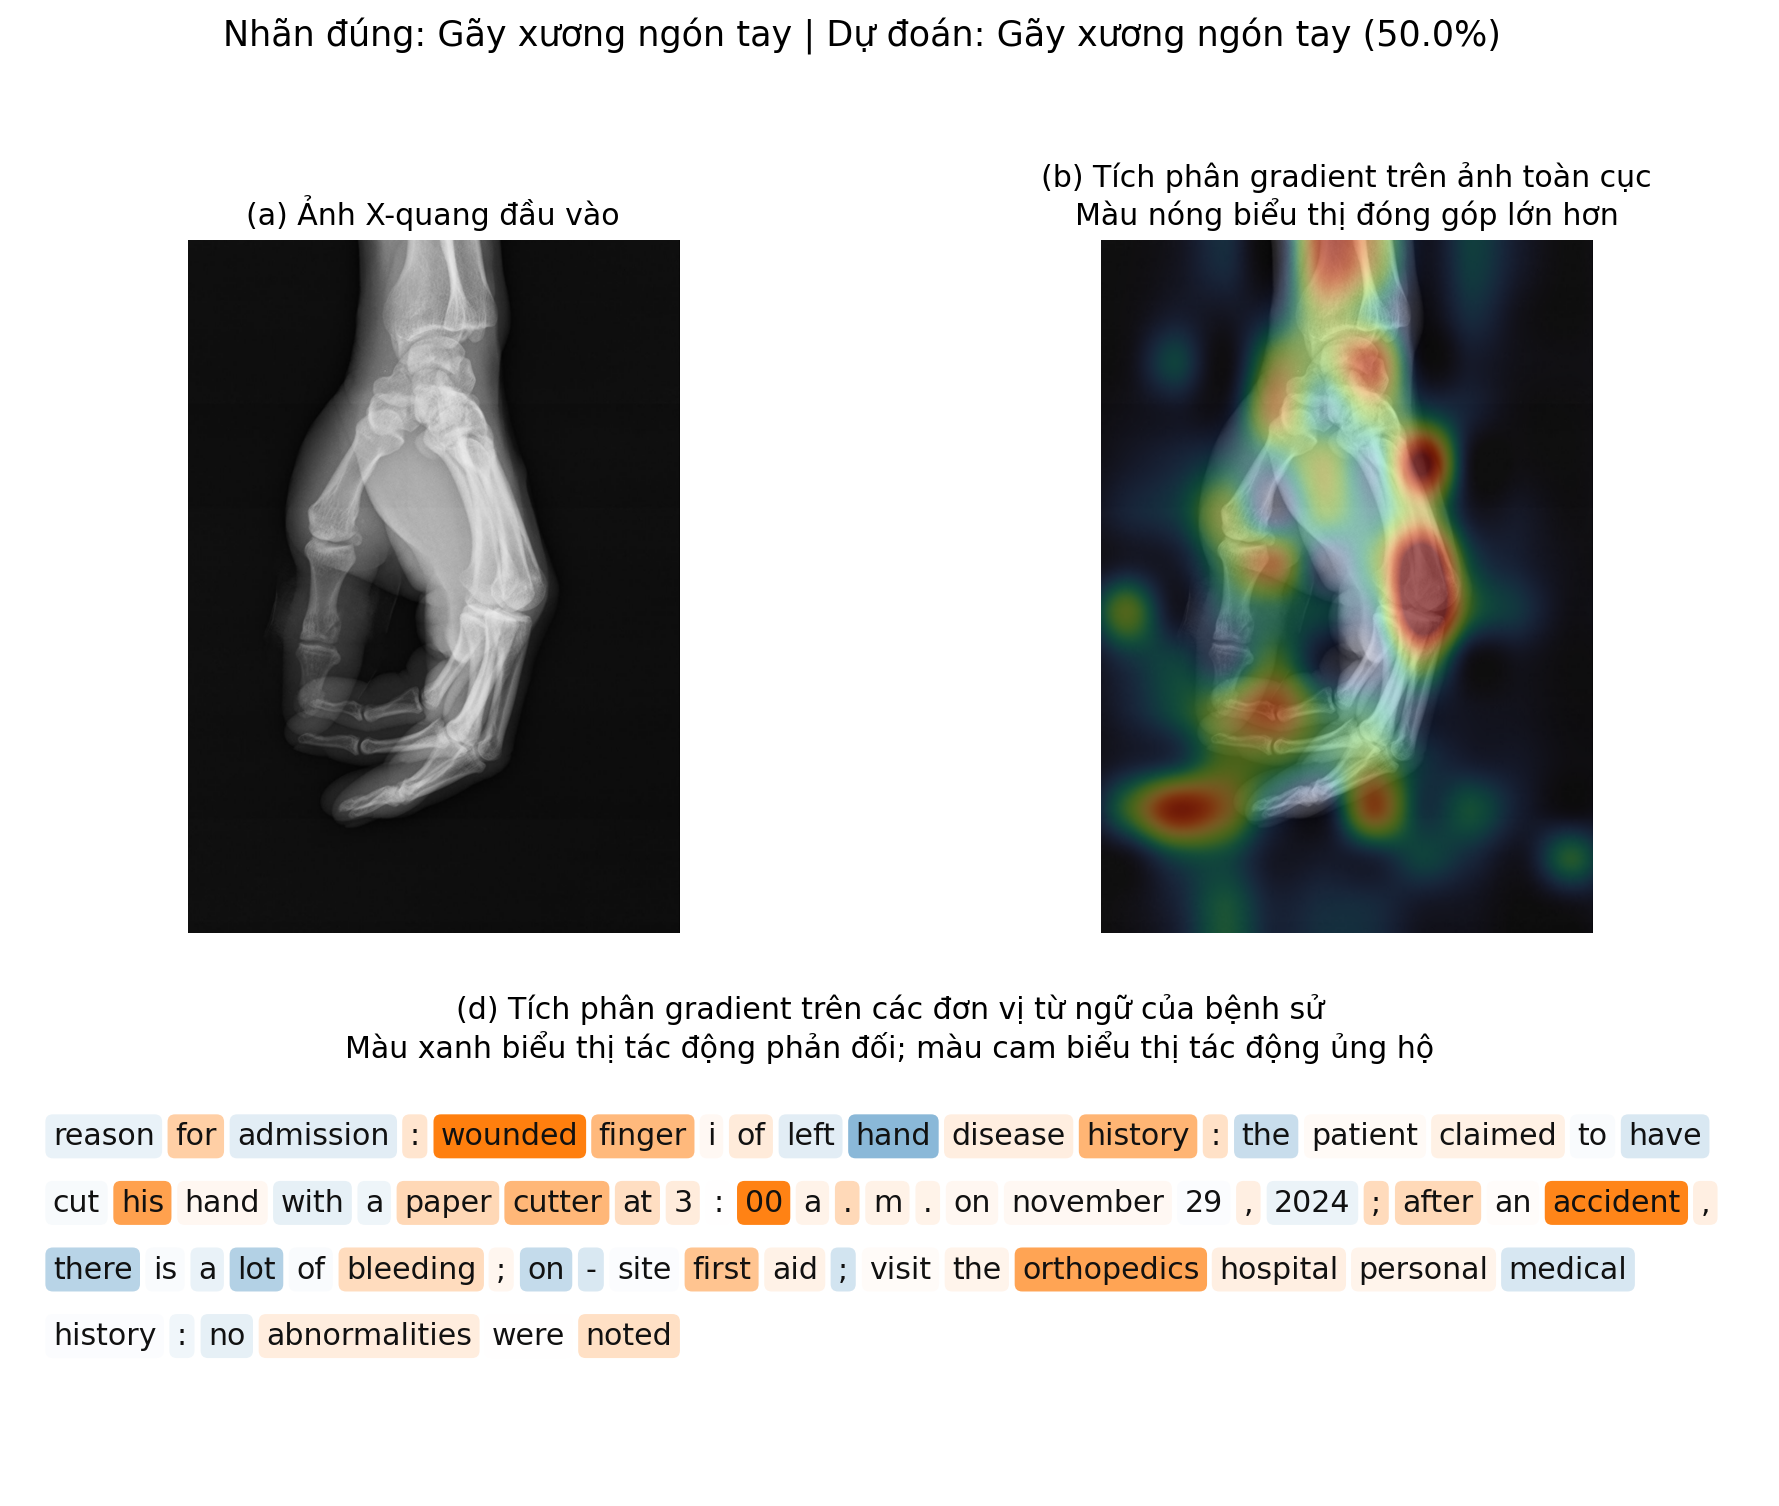
\includegraphics[trim={17.59904bp 111.59392bp 366.78003bp 471.17435bp},clip,width=0.944573\linewidth]{ig_case_source.png}\\[-1pt]
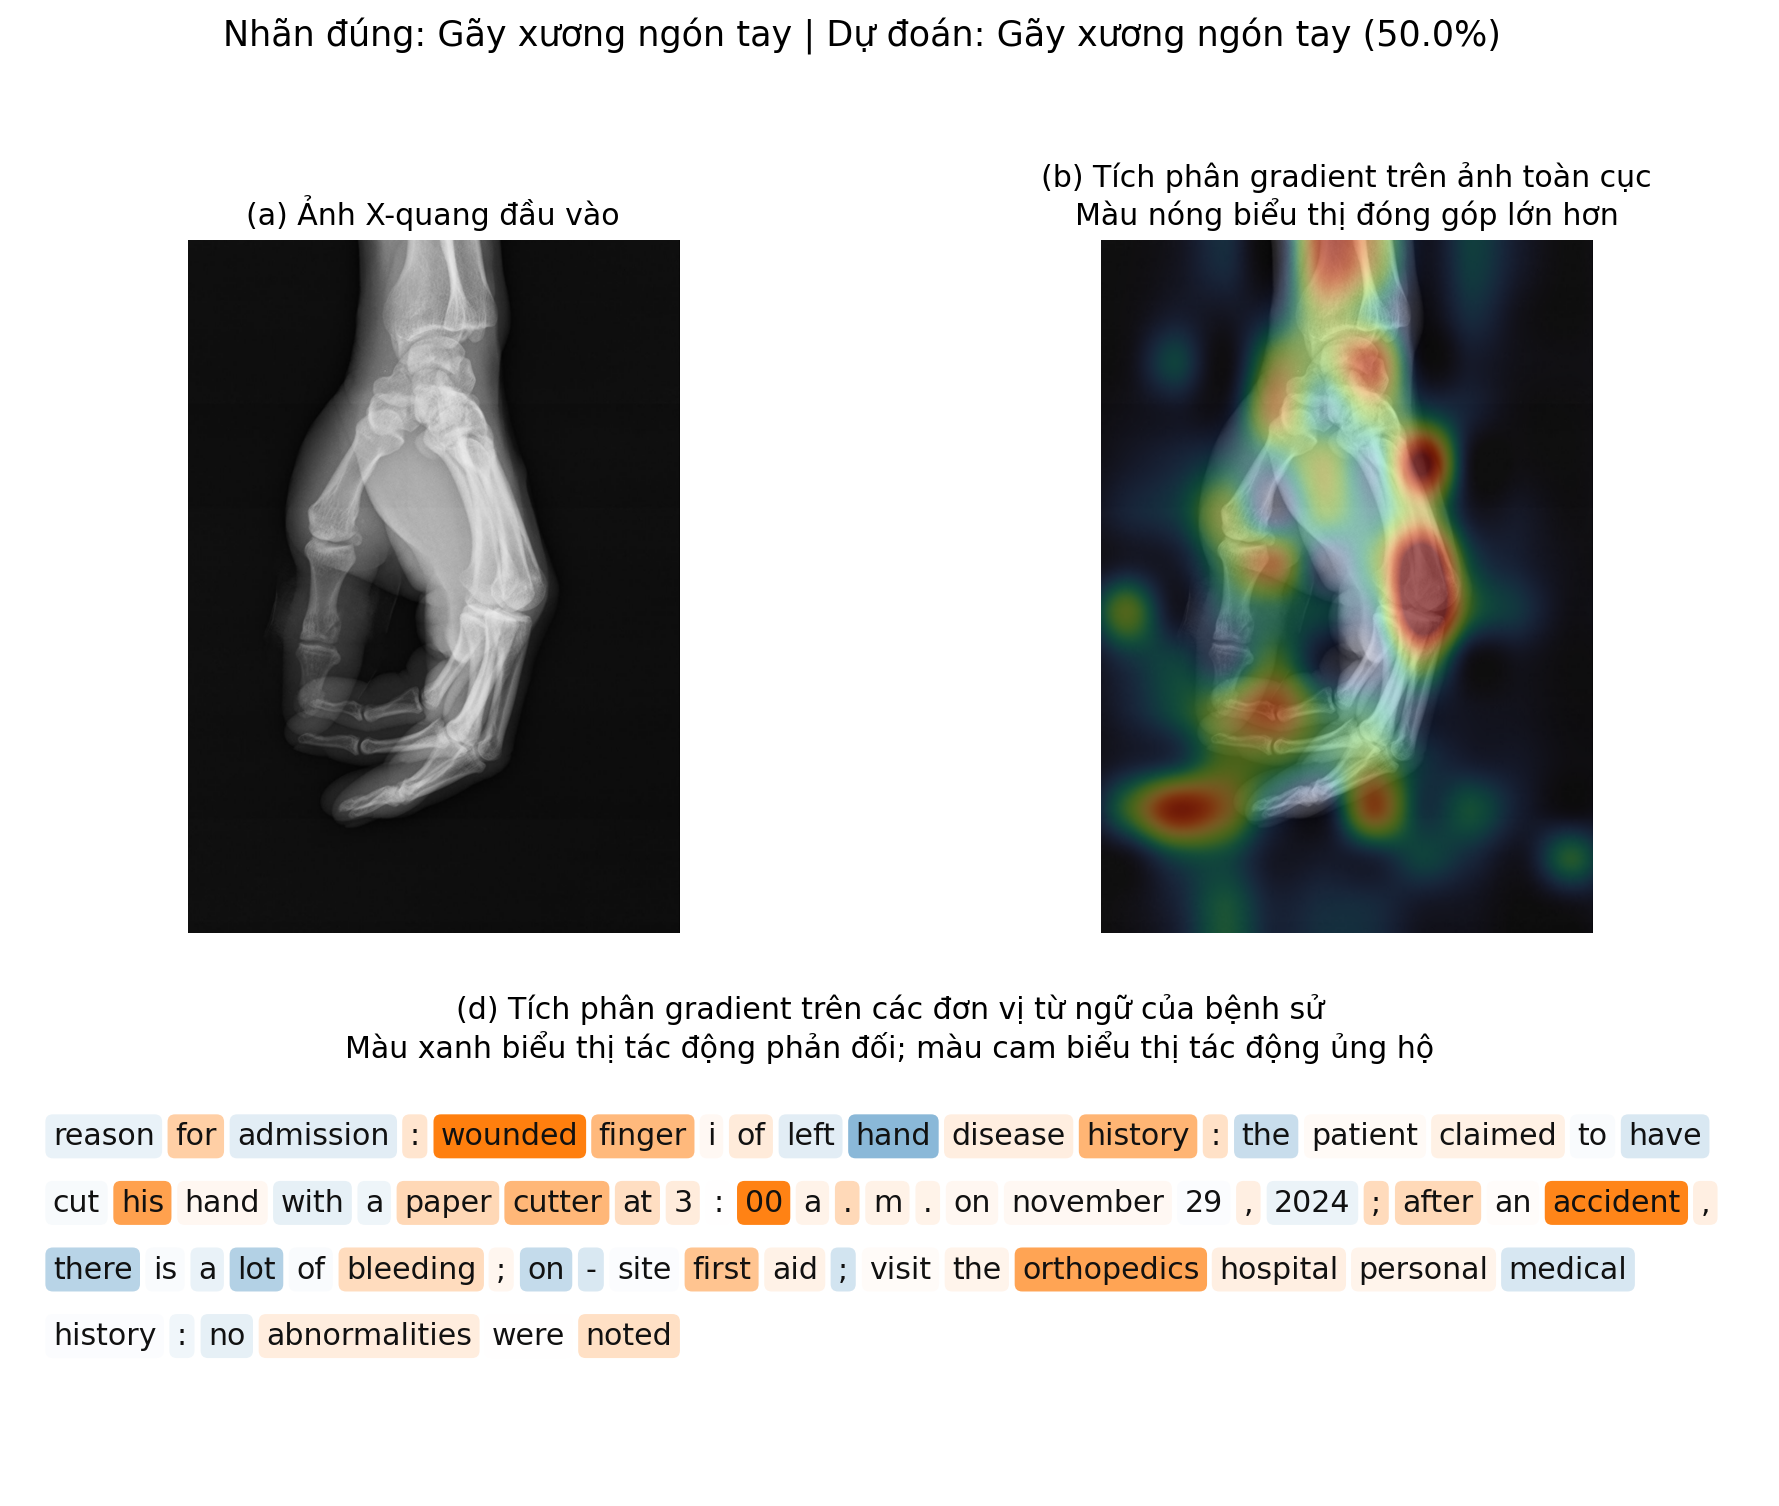
\includegraphics[trim={345.18121bp 111.59392bp 23.59872bp 471.17435bp},clip,width=0.989607\linewidth]{ig_case_source.png}\\[-1pt]
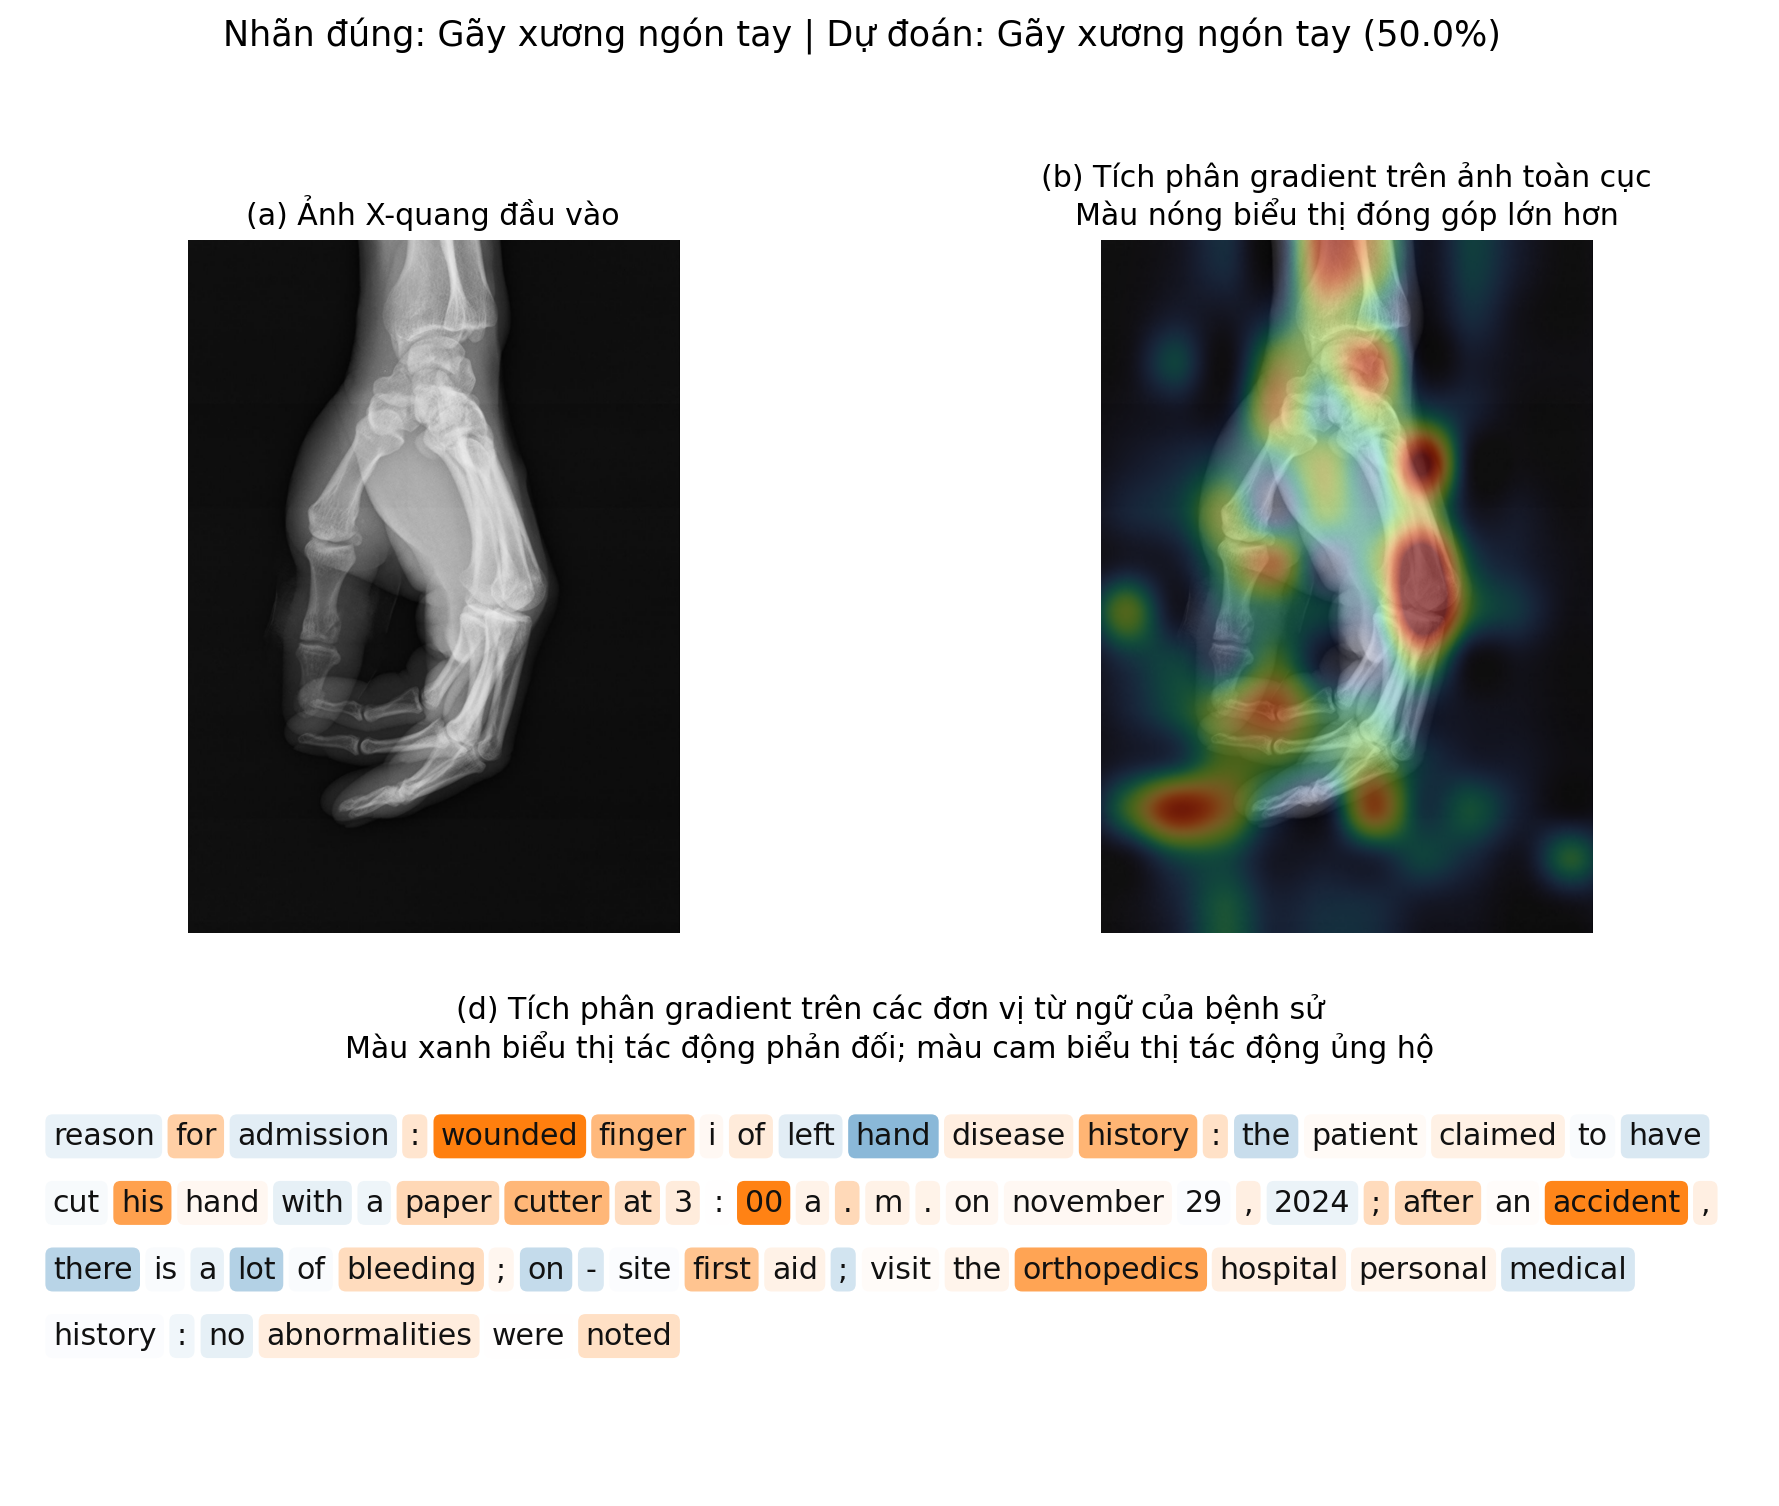
\includegraphics[trim={17.19906bp 84.79538bp 368.37994bp 497.97289bp},clip,width=0.941109\linewidth]{ig_case_source.png}\\[-1pt]
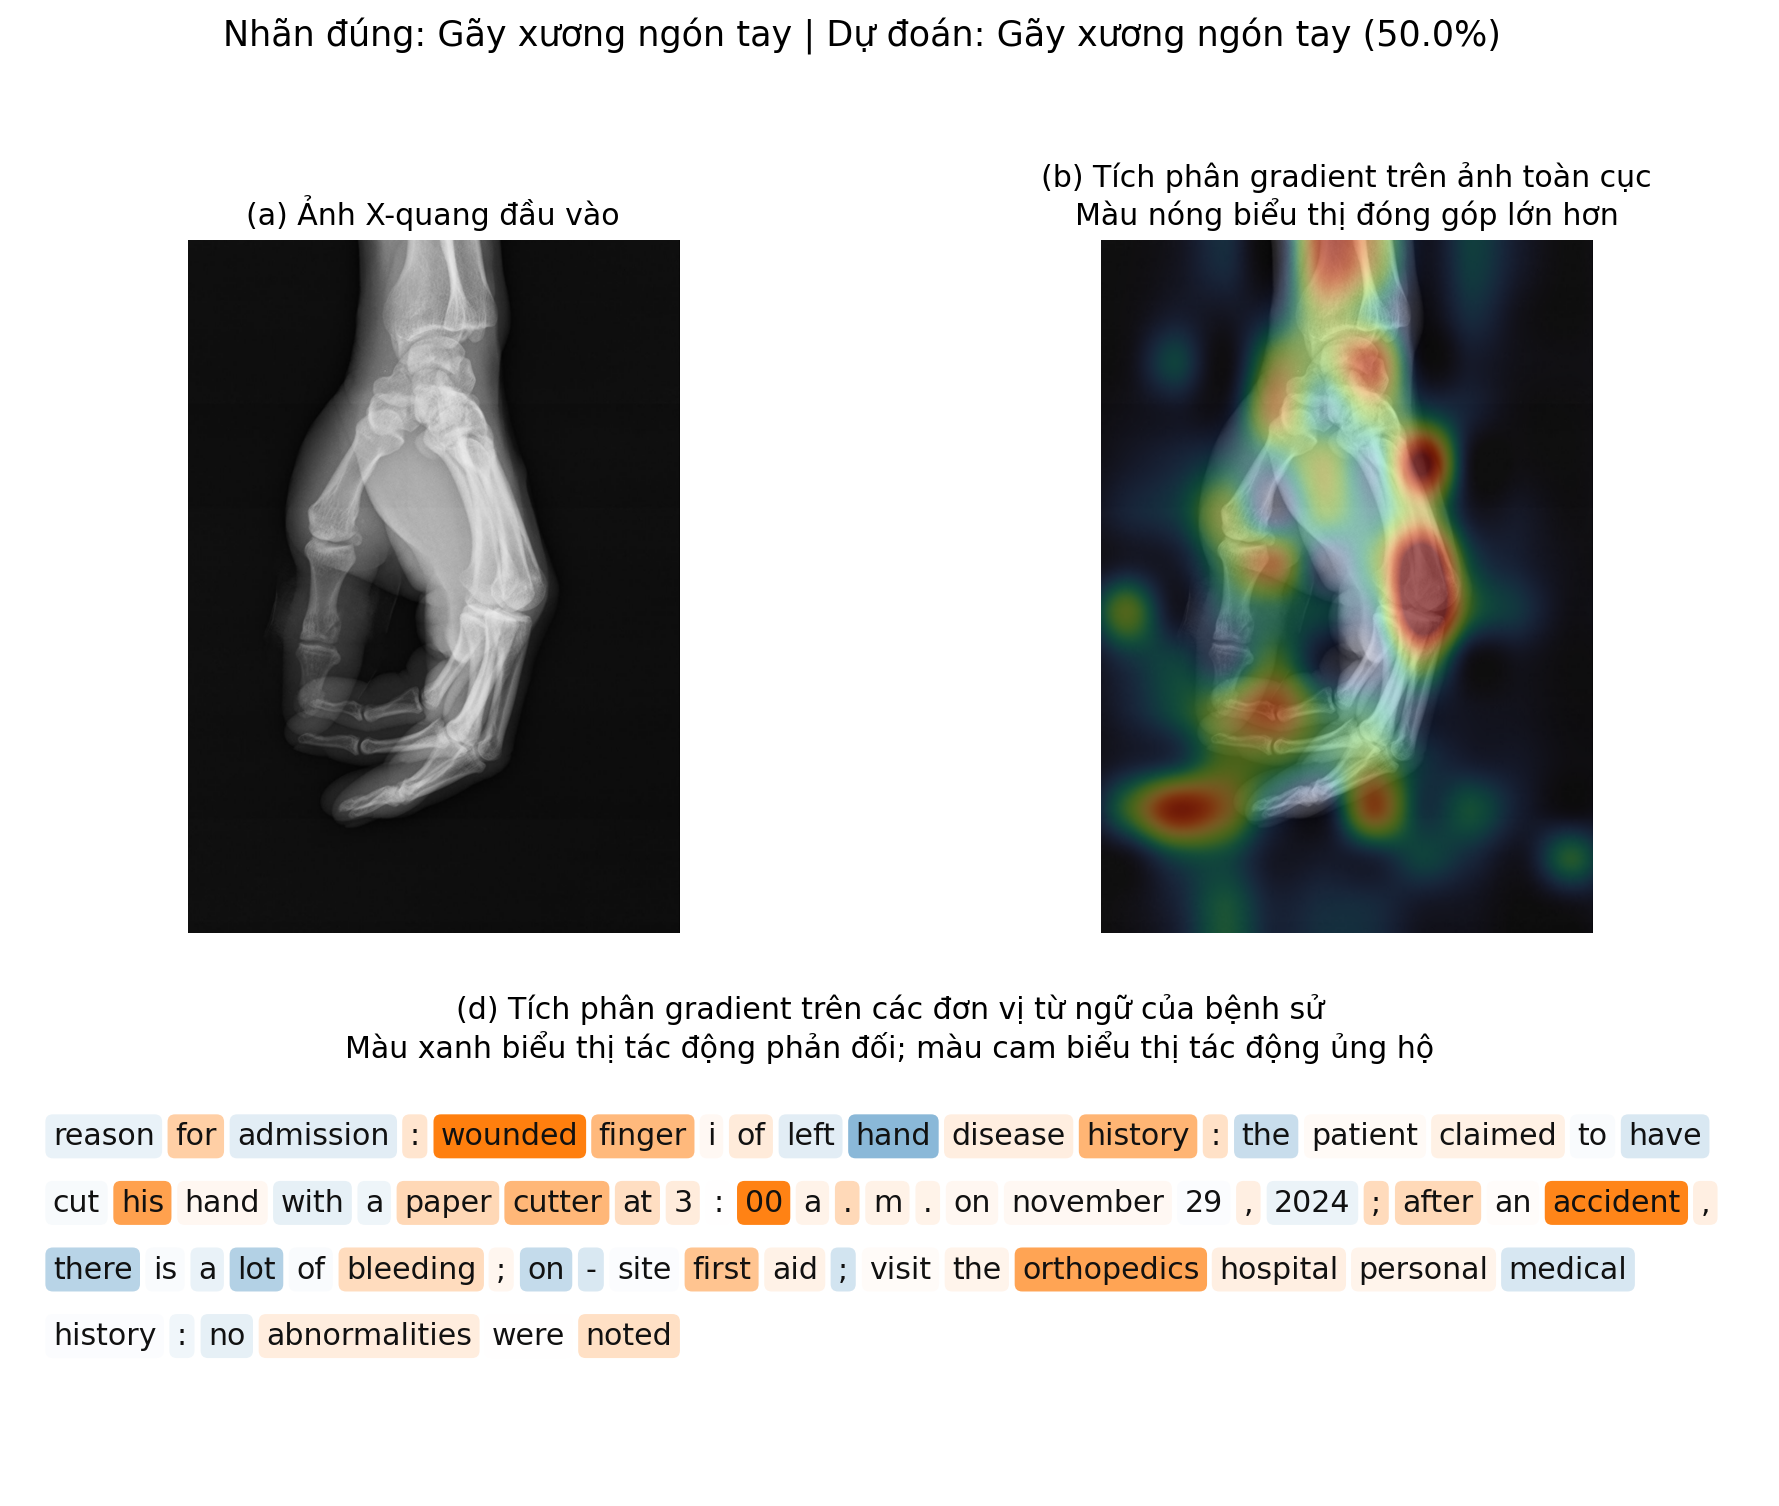
\includegraphics[trim={347.18110bp 84.79538bp 56.79691bp 497.97289bp},clip,width=0.887991\linewidth]{ig_case_source.png}\\[-1pt]
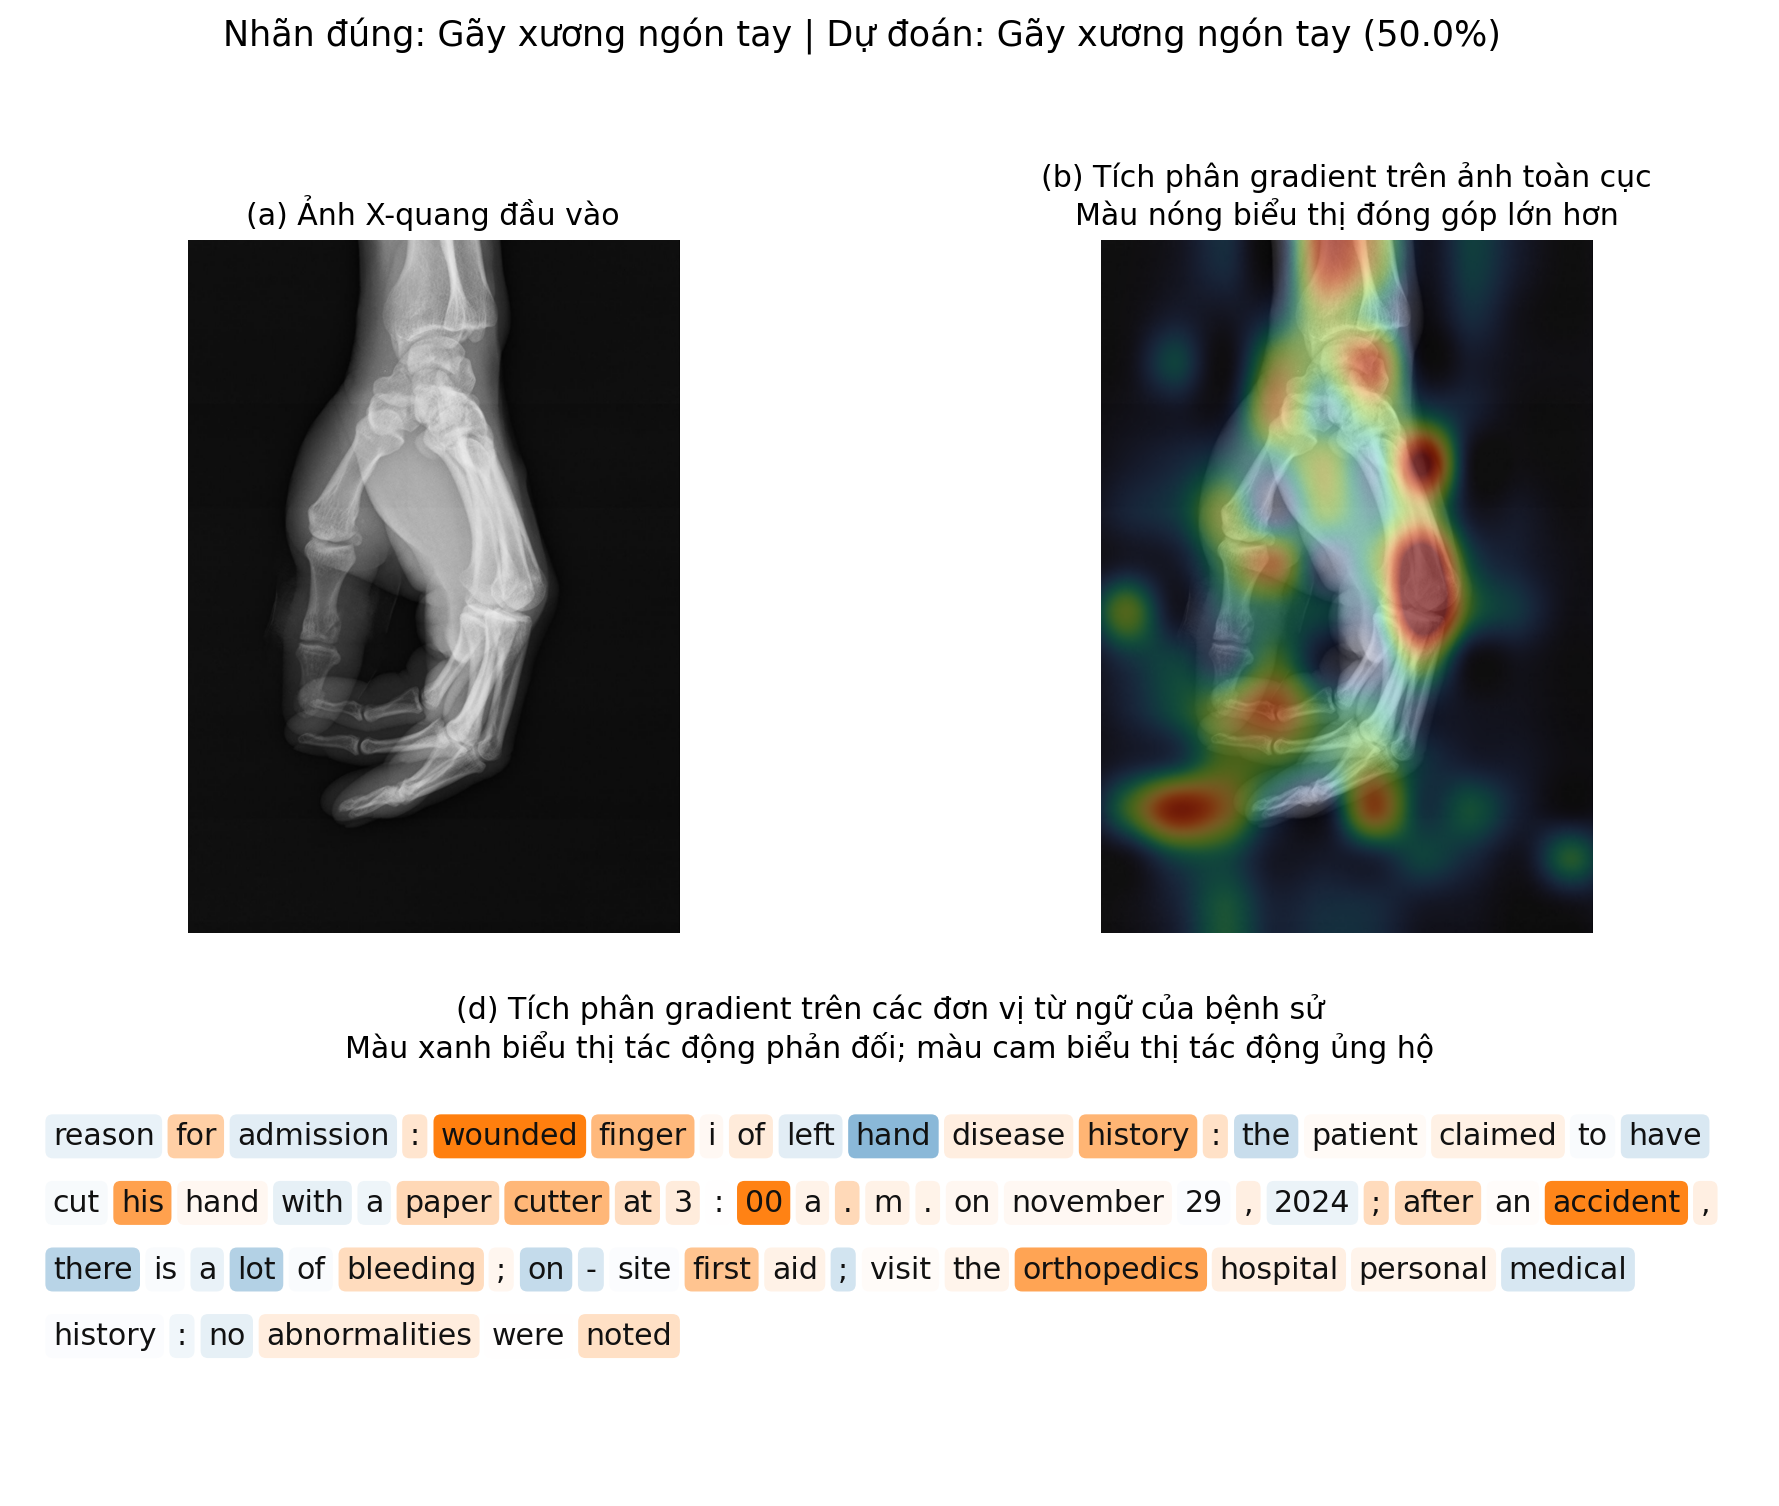
\includegraphics[trim={21.59882bp 58.39682bp 438.77611bp 524.77143bp},clip,width=0.725173\linewidth]{ig_case_source.png}\\[-1pt]
{\scriptsize\textcolor{blue!65!black}{Blue: opposing}\quad
\textcolor{orange!85!black}{Orange: supporting}}
\end{minipage}
\par\endgroup

\caption{Qualitative IG for CTCH case 3563 (XBone-Net, seed 42). Warm image colors indicate greater displayed relevance. Orange and blue text respectively support and oppose the predicted-class logit. Each attribution holds the other modality fixed. This selected example does not establish lesion localization.}
\label{fig:ig_case}
\end{figure*}

\section{Limitations and Conclusion}
XBone-Net combines class-aware alignment, low-rank adaptation, and bidirectional fusion for radiograph--history classification. Across the evaluated datasets, it achieves competitive Macro-F1 while reducing trainable parameters and training memory, with longer training and higher CTCH inference latency. Architecture ablations and input interventions characterize this application-level trade-off.

Fixed splits, three training seeds, single-center CTCH data, and synthetic BTXRD text limit generalization. The IG analysis uses one seed. Direct prompt-learning comparisons, isolated loss/sampler ablations, and independent patient-level validation remain absent. These retrospective results do not establish clinical deployment readiness.

Future work will evaluate independent cohorts and per-class errors, test missing or mismatched histories, and assess IG stability across references and seeds with clinician review. Simplified fusion and model compression should be evaluated jointly against accuracy, memory, and latency.

\bibliographystyle{IEEEtran}
\bibliography{references}
\end{document}
